\documentclass[a4paper]{book}

%% Language and font encodings
%\usepackage{fontspec}
%\setmainfont{Times New Roman}\usepackage{CormorantGaramond}
\usepackage[toc,page]{appendix}
\usepackage[T1]{fontenc}
% \usepackage[utf8x]{inputenc}
\usepackage[utf8]{inputenc}
\usepackage[swedish, english]{babel}
\usepackage{float}
\usepackage[colorlinks=true, allcolors=black]{hyperref}
\usepackage{xcolor}
\usepackage{tikz}
\usepackage{caption}
\usepackage{subcaption}
\usepackage{graphicx}
\usepackage{mathtools}
\urlstyle{tt}
\newcommand{\email}[1]{\href{mailto:#1}{\tt{\nolinkurl{#1}}}}
\newcommand{\orcid}[1]{ORCID: \href{https://orcid.org/#1}{\tt{\nolinkurl{#1}}}}

\usepackage[parfill]{parskip}
\renewcommand*\oldstylenums[1]{\carlitoOsF #1}
% \usepackage{fancyhdr}
%\usepackage{natbib}
\usepackage{authblk}
\setlength{\headheight}{41pt}
\setlength{\textwidth}{440pt}
%\pagestyle{fancy}

%% Sets page size and margins
\usepackage[a4paper,top=3cm,bottom=2cm,left=3cm,right=3cm,marginparwidth=1.75cm]{geometry}

%% Useful packages
\usepackage{graphicx}
\usepackage{booktabs}
\usepackage{caption}
\usepackage{amsmath}
\usepackage{mathtools}

\usepackage{titlesec}
\setcounter{secnumdepth}{4}

\usepackage[colorinlistoftodos]{todonotes}
\usepackage[yyyymmdd]{datetime}
\renewcommand{\dateseparator}{-}
\rmfamily
% \fancyhead[L]{\rmfamily Bi-MMC battery}

\usepackage{xspace}

% \usepackage[utf8]{inputenc}

%% Package to import MATLAB codes
\usepackage{listings}
\lstset{ 
	language=Matlab,                		% choose the language of the code
%	basicstyle=10pt,       				% the size of the fonts that are used for the code
	numbers=left,                  			% where to put the line-numbers
	numberstyle=\footnotesize,      		% the size of the fonts that are used for the line-numbers
	stepnumber=1,                   			% the step between two line-numbers. If it's 1 each line will be numbered
	numbersep=5pt,                  		% how far the line-numbers are from the code
%	backgroundcolor=\color{white},  	% choose the background color. You must add \usepackage{color}
	showspaces=false,               		% show spaces adding particular underscores
	showstringspaces=false,         		% underline spaces within strings
	showtabs=false,                 			% show tabs within strings adding particular underscores
%	frame=single,	                			% adds a frame around the code
%	tabsize=2,                				% sets default tabsize to 2 spaces
%	captionpos=b,                   			% sets the caption-position to bottom
	breaklines=true,                			% sets automatic line breaking
	breakatwhitespace=false,        		% sets if automatic breaks should only happen at whitespace
	escapeinside={\%*}{*)}          		% if you want to add a comment within your code
}

\usepackage{layouts} %% used for textwidth and textheight

\usepackage{matlab}

%% cancelling values
\usepackage[makeroom]{cancel}

%% theorem 
\newtheorem{theorem}{Theorem}

\title{\Large Non-linear $\mathcal{O}$bservers Course}
\author{Arvind Balachandran}
\date{\today}

\begin{document}

\maketitle
\pagenumbering{gobble}
\newpage
\pagenumbering{arabic}

\chapter{Observers for Linear Systems}
\section{Le 1.1}
Model: 
\begin{align*}
    A = \begin{pmatrix}
        \mu_1 & 1 & 0 \\ 0 & \mu_1 & 1 \\ 0 & 0 & \mu_2
    \end{pmatrix}, \quad C = \begin{pmatrix}
        0 & 0 & 1
    \end{pmatrix}
\end{align*}
The observability matrix is 
\begin{align*}
    \mathcal{O} &= \begin{pmatrix}
        C \\ C\,A \\ C\,A^2
    \end{pmatrix} = \begin{pmatrix}
        0 & 0 & 1 \\ 0 & 0 & \mu_2 \\ 0 & 0 & \mu_2^2 
    \end{pmatrix}
\end{align*}
The null space of the observability matrix
\begin{align*}
    \mathcal{N}\left(\mathcal{O}\right) &= \begin{Bmatrix}
        \begin{pmatrix}
            1 \\ 0 \\ 0
        \end{pmatrix},\ \begin{pmatrix}
            0 \\ 1 \\ 0
        \end{pmatrix}
    \end{Bmatrix}
\end{align*}
Considering the following:
\begin{align*}
    \begin{pmatrix}
        \lambda\,I - A \\ C
    \end{pmatrix} = \begin{pmatrix}
        \lambda - \mu_1 & -1 & 0 \\ 0 & \lambda - \mu_1 & -1\\ 0 & 0 & \lambda - \mu_2 \\ 0 & 0 & 1
    \end{pmatrix}
\end{align*}
Substituting $\lambda = \mu_1,\ \mu_2$,
\begin{align*}
    \Lambda_1 &= \begin{pmatrix}
        0 & -1 & 0 \\ 0 & 0 & -1 \\ 0 & 0 & \mu_1 - \mu_2 \\ 0 & 0 & 1
    \end{pmatrix}, & \Lambda_2 = \begin{pmatrix}
        \mu_2 - \mu_1 & -1 & 0 \\ 0 & \mu_2 - \mu_1 & -1\\ 0 & 0 & 0 \\ 0 & 0 & 1
    \end{pmatrix}
\end{align*}
now, 
\begin{align*}
    \mathcal{N}\left(\Lambda_1\right) &= \begin{Bmatrix} \begin{pmatrix}
        1 \\ 0 \\ 0
    \end{pmatrix} \end{Bmatrix} , & \mathcal{N}\left(\Lambda_2\right) &= \begin{Bmatrix} \emptyset \end{Bmatrix}.
\end{align*}
it is clear that $\mathcal{N}\begin{pmatrix}
    \lambda\,I - A \\ C
\end{pmatrix}$ is not the same as $\mathcal{N}\left(\mathcal{O}\right)$, but rather a subset.


\clearpage
\section{Le 1.2}
\begin{align*}
    \dot \theta_1 &= 0 \quad \dot \theta_2 = 0 & z(t) &= \begin{pmatrix}
        1-y(t) & y(t)
    \end{pmatrix}\,\theta \\
    A &= \begin{pmatrix}
        0 & 0 \\
        0 & 0
    \end{pmatrix} & C &= \begin{pmatrix}
        1-y(t) & y(t)
    \end{pmatrix}
\end{align*}
The observability criterion is 
\begin{align*}
    \Sigma_0 &= \int_{0}^{\infty} e^{A^Tt}\,C^T\,C\,e^{At} dt \\
    \Sigma_0 &= \int_{0}^{\infty} e^{\begin{pmatrix} 0 & 0 \\ 0 & 0\end{pmatrix}t}\, \begin{pmatrix} 1-y(t) \\ y(t) \end{pmatrix}\,\begin{pmatrix} 1-y(t) & y(t) \end{pmatrix}\,e^{\begin{pmatrix} 0 & 0 \\ 0 & 0\end{pmatrix}t} dt \\
    \Sigma_0 &= \int_{0}^{\infty} I\, \begin{pmatrix} 1-y(t) \\ y(t) \end{pmatrix}\,\begin{pmatrix} 1-y(t) & y(t) \end{pmatrix}\,I dt \\
    \Sigma_0 &= \int_{0}^{\infty} \begin{pmatrix} \left(1-y(t)\right)^2 & y(t)\,\left(1-y(t)\right)\\ y(t)\,\left(1-y(t)\right) & y^2(t) \end{pmatrix}\,dt \\
    \Sigma_0 &= \begin{pmatrix} \int_{0}^{\infty} \left(1+y^2(t)-2y(t)\right)\,dt & \int_{0}^{\infty} \left(y(t)-y^2(t)\right)\,dt\\ \int_{0}^{\infty} \left(y(t)-y^2(t)\right)\,dt & \int_{0}^{\infty} y^2(t)\,dt \end{pmatrix}
\end{align*}
Let, 
\begin{align*}
    Y_1 &= \int_{0}^{\infty} y(t) dt & \&,\ Y_2 &= \int_{0}^{\infty} y^2(t) dt
\end{align*}
Therefore, 
\begin{align*}
    \Sigma_0 &= \begin{pmatrix} t + Y_2 - 2Y_1 & Y_1 - Y_2\\ Y_1 - Y_2 & Y_2 \end{pmatrix}.
\end{align*}
For the system to be observable det$\left(\Sigma_0\right) \neq 0$, i.e., 
\begin{align*}
    \text{det}\left(\Sigma_0\right) \neq 0 \implies Y_2t + Y_2^2 - 2Y_1Y_2 + \left(Y_1 - Y_2\right)^2 &\neq 0 \\
    Y_2t + \bcancel{Y_2^2} - \cancel{2Y_1Y_2} - Y_1^2 - \bcancel{Y_2^2} + \cancel{2Y_1Y_2} &\neq 0 \\
    Y_2t - Y_1^2 &\neq 0 \\
    t\,\int_{0}^{\infty} y^2(t) dt - \left(\int_{0}^{\infty} y(t) dt\right)^2 &\neq 0 
\end{align*}
If $y(t)$ is a constant then det$\left(\Sigma_0\right) = 0$.

 
\clearpage
\section{Le 1.3}
Show that the observability gramian $\Sigma_o$ satisfies the Lyapunov equation
\begin{align*}
    A^T\,\Sigma_o + \Sigma_o\,A + C^T\,C = 0,
\end{align*}
or, 
\begin{align*}
    A^T\,\Sigma_o + \Sigma_o\,A = - C^T\,C.
\end{align*}
Multiply $e^{At}$ to the right and $e^{A^Tt}$ to the left,
\begin{align*}
    e^{A^Tt}\,A^T\,\Sigma_o\,e^{At} + e^{A^Tt}\,\Sigma_o\,A\,e^{At} = -e^{A^Tt}\,C^T\,C\,e^{At}.
\end{align*}
Since, 
\begin{align*}
    \frac{d}{dt}e^{At} = A\,e^{At}
\end{align*}
as $e^{At}$ and $A$ are commutative, 
\begin{align*}
    \left(\frac{d}{dt}e^{A^Tt}\right)\,\Sigma_o\,e^{At} + e^{A^Tt}\,\Sigma_o\,\left(\frac{d}{dt}e^{At}\right) = -e^{A^Tt}\,C^T\,C\,e^{At}.
\end{align*}
Using the product rule, 
\begin{align*}
    \frac{d}{dt}\left(e^{A^Tt}\,\Sigma_o\,e^{At}\right) = -e^{A^Tt}\,C^T\,C\,e^{At}.
\end{align*}
integrating both sides with limits from 0 to $\infty$
\begin{align*}
    \int_0^\infty\frac{d}{dt}\left(e^{A^Tt}\,\Sigma_o\,e^{At}\right) dt &= \int_0^\infty-e^{A^Tt}\,C^T\,C\,e^{At} dt.\\
    \implies \left[e^{A^Tt}\,\Sigma_o\,e^{At}\right]_0^\infty &= \int_0^\infty-e^{A^Tt}\,C^T\,C\,e^{At} dt.
\end{align*}
for a linear system with the state equation $\dot X = A\,X$ solves to $X = e^{At}$ and 
\begin{align*}
    \lim_{t\to\infty}X = \lim_{t\to\infty}e^{At} = 0
\end{align*}
if the eigenvalues are on the left-hand side of the complex plane.
Using the stability requirement
\begin{align*}
    \left[e^{A^Tt}\,\Sigma_o\,e^{At}\right]_0^\infty &= \int_0^\infty-e^{A^Tt}\,C^T\,C\,e^{At} dt.\\
    \text{becomes, } \Sigma_o &= \int_0^\infty e^{A^Tt}\,C^T\,C\,e^{At} dt.
\end{align*}
\clearpage
\section{Le 1.4} 
Compute the observability gramian as a function of $\mathbf{\epsilon}$ and interpret the result.
\newcommand{\gramian}{\begin{pmatrix}
    \sigma_{1} & \sigma_{2} \\
    \sigma_{2} & \sigma_{3}
\end{pmatrix}}

\begin{align*}
    \dot x &= \begin{pmatrix}
        -2 & -1 \\
        \epsilon & -1
    \end{pmatrix}\,x \\
    y &= \begin{pmatrix}
        1 & 1
    \end{pmatrix}\,x
\end{align*}

the gramian is given as
\begin{align}
    \Sigma_o = \int_{0}^{\infty} \exp\left(A^Tt\right)\,C^T\,C\,\exp\left(At\right) dt = \int_{0}^{\infty} \mathcal{X} dt \label{eq:le41}
\end{align}

or the solution to the Lyapunov equation,
\begin{align*}
    A^T\,\Sigma_o + \Sigma_o\,A + C^T\,C = 0,
\end{align*}
substituing $A$ and $C$, 
\begin{align*}
    \begin{pmatrix}
        -2 & -1 \\
        \epsilon & -1
    \end{pmatrix}^T\,\Sigma_o + \Sigma_o\,\begin{pmatrix}
        -2 & -1 \\
        \epsilon & -1
    \end{pmatrix} + \begin{pmatrix}
        1 & 1
    \end{pmatrix}^T\,\begin{pmatrix}
        1 & 1
    \end{pmatrix} &= 0,\\
    \begin{pmatrix}
        -2 & -1 \\
        \epsilon & -1
    \end{pmatrix}^T\,\Sigma_o + \Sigma_o\,\begin{pmatrix}
        -2 & -1 \\
        \epsilon & -1
    \end{pmatrix} &= - \begin{pmatrix}
        1 & 1 \\
        1 & 1
    \end{pmatrix},\\
\end{align*}
Let, 
\begin{align*}
    \Sigma_o = \gramian,
\end{align*}
then, 
\begin{align*}
    \begin{pmatrix}
        -2 & \epsilon \\
        -1 & -1
    \end{pmatrix}\,\gramian + \gramian\,\begin{pmatrix}
        -2 & -1 \\
        \epsilon & -1
    \end{pmatrix} + \begin{pmatrix}
        1 & 1 \\
        1 & 1
    \end{pmatrix}, &= 0\\
    \implies \begin{pmatrix}
        \epsilon\,\sigma_2 - 2\sigma_1 & \epsilon\,\sigma_3 - 2\sigma_2 \\
        -\sigma_1 - \sigma_2 & - \sigma_2 - \sigma_3
    \end{pmatrix} + \begin{pmatrix}
        \epsilon\,\sigma_2 - 2\sigma_1 & -\sigma_1 - \sigma_2 \\
        \epsilon\,\sigma_3 - 2\sigma_2 & - \sigma_2 - \sigma_3
    \end{pmatrix} + \begin{pmatrix}
        1 & 1 \\
        1 & 1
    \end{pmatrix}, &= 0\\
    \implies \begin{pmatrix}
        2\epsilon\,\sigma_2 - 4\sigma_1 & \epsilon\,\sigma_3 - 3\sigma_2 - \sigma_1 \\
        \epsilon\,\sigma_3 - 3\sigma_2 - \sigma_1 & 2\sigma_2 - 2\sigma_3
    \end{pmatrix} + \begin{pmatrix}
        1 & 1 \\
        1 & 1
    \end{pmatrix}, &= 0\\
    \implies \begin{pmatrix}
        2\epsilon\,\sigma_2 - 4\sigma_1 + 1 & \epsilon\,\sigma_3 - 3\sigma_2 - \sigma_1 + 1\\
        \epsilon\,\sigma_3 - 3\sigma_2 - \sigma_1 + 1 & 2\sigma_2 - 2\sigma_3 + 1
    \end{pmatrix}  &= 0,\\
    \implies 2\epsilon\,\sigma_2 - 4\sigma_1 + 1 &= 0 \\
    \epsilon\,\sigma_3 - 3\sigma_2 - \sigma_1 + 1 &= 0\\
    2\sigma_2 - 2\sigma_3 + 1 &= 0.\\
    \Sigma_o = \frac{1}{6\,\left(\epsilon + 2\right)}\,\begin{pmatrix}
        \epsilon^2 + 3\,\epsilon + 3 & 2\,\epsilon + 3  \\
        2\,\epsilon + 3 & \epsilon + 3
    \end{pmatrix}
\end{align*}
For $\Sigma_o$ to have full-rank, $\det\left(\Sigma_o\right) \neq 0$, i.e., 
\begin{align*}
    \frac{1}{6\,\left(\epsilon + 2\right)} &\neq 0, & \text{i.e., } \epsilon^2 + \epsilon &\neq 0
\end{align*}
For $\epsilon = -2$, $\Sigma_o$ is signular.

For $\epsilon = 0$, rank$\left(\Sigma_o\right) = 1$. 

% $\Sigma_o$ is full-column rank for $\epsilon \neq 0 $ and $\epsilon \neq -\frac{36}{25} $.

% i.e., 
% \begin{align*}
%     -4\,\Sigma_{11} + \epsilon\,\Sigma_{21} + \epsilon\,\Sigma_{12} + 1 &= 0\\
%     -3\,\Sigma_{12} + \epsilon\,\Sigma_{22} -\Sigma_{11} + 1 &= 0\\
%     -\Sigma_{11} -3\,\Sigma_{21} + \epsilon\,\Sigma_{22} + 1 &= 0\\
%     -\Sigma_{12} -2\,\Sigma_{22} -\Sigma_{21} + 1 &= 0
% \end{align*}
% substituing $A$ and $C$, 
% \begin{align*}
%     \mathcal{X} &= \exp\left(\begin{pmatrix}
%         -2 & \epsilon \\
%         -1 & -1
%     \end{pmatrix}t\right)\,\begin{pmatrix}
%         1 \\
%         1
%     \end{pmatrix}\,\begin{pmatrix}
%         1 & 1
%     \end{pmatrix}\,\exp\left(\begin{pmatrix}
%         -2 & -1 \\
%         \epsilon & -1
%     \end{pmatrix}t\right) \\
%     &= \begin{pmatrix}
%         \exp\left(-2t\right) + \exp\left(t\epsilon^*\right) \\
%         2\exp\left(-t\right)
%     \end{pmatrix}\,\begin{pmatrix}
%         1 & 1
%     \end{pmatrix}\,\exp\left(\begin{pmatrix}
%         -2 & -1 \\
%         \epsilon & -1
%     \end{pmatrix}t\right) \\
%     &= \begin{pmatrix}
%         \exp\left(-2t\right) + \exp\left(t\epsilon^*\right) & \exp\left(-2t\right) + \exp\left(t\epsilon^*\right) \\
%         2\exp\left(-t\right) & 2\exp\left(-t\right)
%     \end{pmatrix}\,\exp\left(\begin{pmatrix}
%         -2 & -1 \\
%         \epsilon & -1
%     \end{pmatrix}t\right) \\
%     &= \begin{pmatrix}
%         e^{-4t}\,\left(e^{t\left(\epsilon + 2\right))} + 1\right)\,\left(e^{t\left(\epsilon^* + 2\right))} + 1\right) & %% exp(-4*t)*(exp(t*(epsilon + 2)) + 1)*(exp(t*(conj(epsilon) + 2)) + 1)
%         2e^{-t}\,\left(e^{t\epsilon^*} + e^{-2t}\right) \\
%         2e^{-3t}\,\left(e^{t\left(\epsilon + 2\right)} + 1\right) & 4e^{-2t}
%     \end{pmatrix} 
% \end{align*}
% \eqref{eq:le41} becomes
% \begin{align}
%     \Sigma_o &= \begin{pmatrix}
%         \int_{0}^{\infty} e^{-4t}\,\left(e^{t\left(\epsilon + 2\right))} + 1\right)\,\left(e^{t\left(\epsilon^* + 2\right))} + 1\right)\,dt & %% exp(-4*t)*(exp(t*(epsilon + 2)) + 1)*(exp(t*(conj(epsilon) + 2)) + 1)
%         \int_{0}^{\infty} 2e^{-t}\,\left(e^{t\epsilon^*} + e^{-2t}\right) \,dt\\
%         \int_{0}^{\infty} 2e^{-3t}\,\left(e^{t\left(\epsilon + 2\right)} + 1\right)\,dt & 
%         \int_{0}^{\infty} 4e^{-2t}\,dt 
%     \end{pmatrix} \nonumber\\
%     &= \begin{pmatrix}
%         \left[\sigma_1\right]_0^\infty & \left[\sigma_2\right]_0^\infty\\
%         \left[\sigma_3\right]_0^\infty & 
%         \left[-2e^{-2t}\right]_0^\infty % \left[\right]_0^\infty
%     \end{pmatrix} = \begin{pmatrix}
%         \left[\sigma_1\right]_0^\infty & \left[\sigma_2\right]_0^\infty\\
%         \left[\sigma_3\right]_0^\infty & 2
%     \end{pmatrix}, \label{eq:le42}
% \end{align}
% where
% \begin{align*}
%     \sigma_1 &= \frac{e^{t\left(\epsilon^* - 2\right)}}{\epsilon^* - 2} - \frac{e^{-4t}}{4} + \frac{e^{t\left(\epsilon - 2\right)}}{\epsilon - 2} + \frac{e^{\left(t\,\left(\epsilon^2 + |\epsilon|^2\right)\right)/\epsilon}}{2\Re{\left(\epsilon\right)}}\\
%     \sigma_2 &= \frac{2e^{t\left(\epsilon - 1\right)}}{\epsilon - 1} - \frac{2e^{-3t}}{3} \\
%     \sigma_3 &= \frac{2e^{t\left(\epsilon^* - 1\right)}}{\epsilon^* - 1} - \frac{2e^{-3t}}{3}
% \end{align*}
% and 
% \begin{align*}
%     \left[\sigma_1\right]_0^\infty &= \left[\frac{e^{t\left(\epsilon^* - 2\right)}}{\epsilon^* - 2}\right]_0^\infty + \frac{1}{4} + \left[\frac{e^{t\left(\epsilon - 2\right)}}{\epsilon - 2}\right]_0^\infty + \left[\frac{e^{\left(t\,\left(\epsilon^2 + |\epsilon|^2\right)\right)/\epsilon}}{2\Re{\left(\epsilon\right)}}\right]_0^\infty &
%     \left[\sigma_2\right]_0^\infty &= \left[\frac{2e^{t\left(\epsilon - 1\right)}}{\epsilon - 1}\right]_0^\infty + \frac{2}{3} \\
%     \left[\sigma_3\right]_0^\infty &= \left[\frac{2e^{t\left(\epsilon^* - 1\right)}}{\epsilon^* - 1}\right]_0^\infty + \frac{2}{3} & & .
% \end{align*}
% Assuming $\epsilon < 2, \epsilon \neq 0$, and is real,
% \begin{align*}
%     \left[\sigma_1\right]_0^\infty &= \frac{1}{4} - \frac{2}{\epsilon - 2} - \frac{1}{2\epsilon} &
%     \left[\sigma_2\right]_0^\infty &= \frac{2}{3} - \frac{2}{\epsilon - 1}\\
%     \left[\sigma_3\right]_0^\infty &= \frac{2}{3} - \frac{2}{\epsilon - 1} & & .
% \end{align*}
% Substituting in \eqref{eq:le42}, the rank is 2 (full column rank).
\clearpage
\section{Le 1.5}
Considering partitioned state equations 
\begin{align*}
    \begin{pmatrix}
        \dot x_r \\ \dot x_n 
    \end{pmatrix} &= \begin{pmatrix}
        A_r & a_r \\ a_n & a_{nn} 
    \end{pmatrix}\,\begin{pmatrix}
        x_r \\ x_n 
    \end{pmatrix} + \begin{pmatrix}
        b_r \\ b_u 
    \end{pmatrix}\,u(t) & y &= x_n
\end{align*} 
This gives, 
\begin{align*}
    \dot x_r &= A_r\,x_r + a_r\,x_n + b_r\,u(t) & \dot x_n &= a_n\,x_r + a_{nn}\,x_n + b_n\,u(t)
\end{align*}
Considering 
\begin{align*}
    y_r &= \dot y - a_{nn}\,y - b_n\,u(t).
\end{align*}
Then, 
\begin{align*}
    \dot x_r &= A_r\,x_r + a_r\,x_n + b_r\,u(t) & y_r &= a_n\,x_r
\end{align*}
The observer is 
\begin{align*}
    \hat x_r &= A_r\,\hat x_r + a_r\,\hat x_n + b_r\,u(t) + K\,\left(y_r - a_n\,\hat x_r\right)
\end{align*}
Substituting $x_n = \hat x_n = y$,
\begin{align*}
    \dot x_r &= A_r\,x_r + a_r\,y + b_r\,u(t) \\
    \dot{\hat x}_r &= A_r\,\hat x_r + a_r\,y + b_r\,u(t) + K\,\left(a_n\,x_r - a_n\,\hat x_r\right)
\end{align*}
The error signal,
\begin{align*}
    \dot{\tilde x}_r &= \dot x_r - \dot{\hat x}_r \\
    &= A_r\,x_r + \cancel{a_r\,y} + \bcancel{b_r\,u(t)} - A_r\,\hat x_r - \cancel{a_r\,y} - \bcancel{b_r\,u(t)} - K\,\left(a_n\,\hat x_r - a_n\,\hat x_r\right) \\
    &= A_r\,x_r - A_r\,\hat x_r - K\,\left(a_n\,x_r - a_n\,\hat x_r\right) \\
    & = \left(A_r - K\,a_n\right)\,\tilde{x}_r
\end{align*}
The poles can be selected arbitrarily in the error dynamics of the reduced observer.
\clearpage
\section{Le 1.6}

\begin{align*}
    X &= \begin{pmatrix}
        0 & 1 \\ 0 & 0
    \end{pmatrix}\,X, \\
    Y &= \begin{pmatrix}
        1 & 0 
    \end{pmatrix}\,X
\end{align*}

Also, 
\begin{align*}
    \alpha_\mathcal{O}(s) = \text{det}\left(SI - A + K\,C\right) &= \det\left[\begin{pmatrix}
        s & 0 \\ 0 & s
    \end{pmatrix} - \begin{pmatrix}
        0 & 1 \\ 0 & 0
    \end{pmatrix} + \begin{pmatrix}
        k_1 \\ k_2
    \end{pmatrix}\,\begin{pmatrix}
        1 & 0
    \end{pmatrix}\right] \\
    &= \det\left[\begin{pmatrix}
        s + k_1 & -1 \\ k_2 & s
    \end{pmatrix}\right] \\
    &= s^2 + k_1\,s + k_2
\end{align*}

The closed-loop observer poles are at $\omega_\alpha$, i.e., 
\begin{align*}
    \alpha_\mathcal{O}(s) &= \left(s + \omega_\alpha\right)\,\left(s + \omega_\alpha\right) = s^2 + 2\,\omega_\alpha\,s + \omega_\alpha^2
\end{align*}

Therefore,
\begin{align*}
    K = \begin{pmatrix}
        k_1 \\ k_2
    \end{pmatrix} = \begin{pmatrix}
        2\omega_\alpha \\ \omega_\alpha^2
    \end{pmatrix}
\end{align*}

The figure below gives the simulation of the full-order observer with the poles at $\omega_\alpha = 5$\,rad/s. 

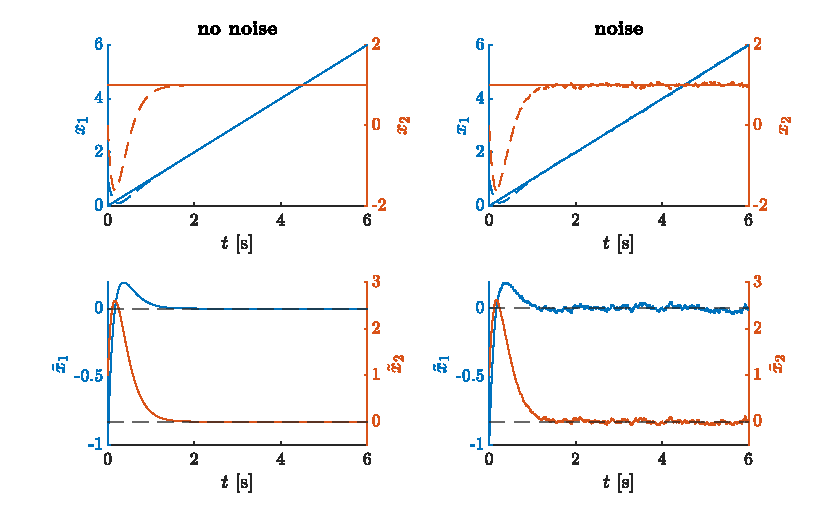
\includegraphics{figures/ex6_p1.pdf}

the blue and orange colors represent the states $x_1$ and $x_2$ respectively, the true state is shown by a solid line, and the estimated state is shown by a dashed line. 

\emph{The reduced state observer} is given as 
\begin{align*}
    \dot w &= \left(0 - l\right)\,w + \left(0 + 0 - 0 - l\,1\,l\right)\,y, & \hat x_1 &= y, \quad \hat x_2 = w + l\,y, \\
    \dot w &= -l\,w - l^2\,y, & \hat x_1 &= y, \quad \hat x_2 = w + l\,y, 
\end{align*}

The figure below gives the simulation of the full-order observer with the poles at $l = 5$\,rad/s. (placing the poles similar to the full-order observer)

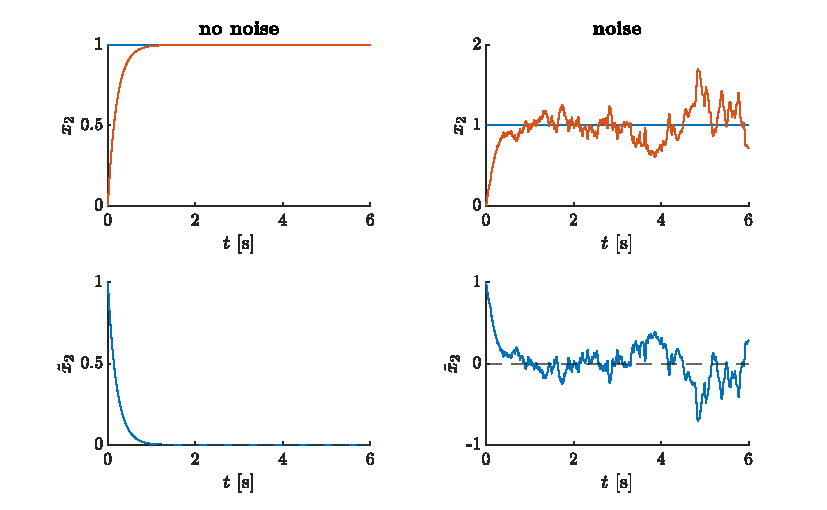
\includegraphics{figures/ex6_p2.pdf}

\fbox{
    \parbox{0.95\textwidth}{
        With the reduced order observer, the noise directly affects the observed 'state' since $x \propto y$ but in the full order observer, the noise is filtered since $\dot x \propto y$.
    }
}

\subsection*{Code}
\begin{matlabcode}
% states 
A = [0 1; 0 0];
C = [1, 0];
system = @(t,y) A*y;

% simulation 
y0 = [0; 1];
tspan = linspace(0,6,5000);
[t_true,y_true] = ode45(@(t,y) system(t,y),tspan,y0);
% adding noise
y_noise = y_true(:,1) + (rand(size(t_true)) - 0.5)*0.5;

% simulation of full-order observer
y0 = [1; 0];
y_val = @(t) interp1(t_true, y_true(:,1), t, 'spline');
[t_fo,y_fo] = ode45(@(t,y) full_order(y,y_val(t),A,C), tspan, y0);
y_temp = interp1(t_true, y_true, t_fo, 'spline');
e_fo = y_temp - y_fo;

% simulation of full-order observer with noise
y_valN = @(t) interp1(t_true, y_noise(:,1), t, 'spline');
[t_foN,y_foN] = ode45(@(t,y) full_order(y,y_valN(t),A,C), tspan, y0);
y_temp = interp1(t_true, y_true, t_foN, 'spline');
e_foN = y_temp - y_foN;

% simulation of reduced-order observer 
y0 = 0;
[t_ro,w] = ode45(@(t,y) reduced_order(y,y_val(t)),tspan,y0);
x2hat = w + 5 * y_val(t_ro);
y_temp = interp1(t_true, y_true(:,2), t_ro, 'spline');
e_ro = y_temp - x2hat;

% simulation of reduced-order observer (with noise)
[t_roN,w] = ode45(@(t,y) reduced_order(y,y_valN(t)),tspan,y0);
x2hatN = w + 5 * y_val(t_roN);
y_temp = interp1(t_true, y_true(:,2), t_roN, 'spline');
e_roN = y_temp - x2hatN;

%% functions
function xdot = full_order(x,y,A,C)
    K = [2*5; 5^2]; % feedback gain 
    xdot = A * x + K*(y - C * x);
end

function wdot = reduced_order(w,y)
    L = 5; % feedback gain 
    wdot = -L * w - L^2 * y;
end
\end{matlabcode}
\clearpage
\section{Kailath 2.3-1a} 

If 
\begin{align*}
    \mathcal{O}_1\,T = \mathcal{O}_2, 
\end{align*}
then 
\begin{align*}
    c_1\,T &= c_2, & c_1\,A_1\,T &= c_2\,A_2 = c_1\,T\,A_2.
\end{align*}
Multiplying $T^{-1}$ on both sides to the right
\begin{align*}
    c_1\,A_1\,T\,T^{-1} &= c_1\,T\,A_2\,T^{-1} & \implies c_1\,A_1 &= c_1\,T\,A_2\,T^{-1}.
\end{align*}
Multiplying $c_1^{-1}$ on both sides to the left
\begin{align*}
    c_1^{-1}c_1\,A_1 &= c_1^{-1}c_1\,T\,A_2\,T^{-1} & \implies A_1 &= T\,A_2\,T^{-1}.
\end{align*}
This is not possible because $c_1$ is not invertible.

The non-observable states cannot be identified but if we measure all states then $A_1$ and $A_2$ will have similar dynamics. 
\section{Kilath 2.3.3}
Realizing linear system to state-space
\begin{align*}
    y &= e\,\frac{s+1}{s\left(s+3\right)} \\ y &= \left(u - y\frac{k}{s+a}\right)\,\frac{s+1}{s\left(s+3\right)} \\ 
    y &= u\,\frac{s+1}{s\left(s+3\right)} - y\,\frac{k\,\left(s+1\right)}{s\left(s+3\right)\left(s+a\right)}\\
    y + y\,\frac{k\,\left(s+1\right)}{s\left(s+3\right)\left(s+a\right)} &= u\,\frac{s+1}{s\left(s+3\right)} \\
    y\,\frac{s\left(s+3\right)\left(s+a\right) + k\,\left(s+1\right)}{s\left(s+3\right)\left(s+a\right)} &= u\,\frac{s+1}{s\left(s+3\right)}\\
    y\,\frac{s\left(s+3\right)\left(s+a\right) + k\,\left(s+1\right)}{\left(s+a\right)} &= u\,\left(s+1\right) \\
    y\,s\left(s+3\right)\left(s+a\right) + y\,k\,\left(s+1\right) &= u\,\left(s+1\right)\,\left(s+a\right)\\
    y\,s\left(s^2+s\left(3+a\right)+3a\right) + y\,k\,\left(s+1\right) &= u\,\left(s^2+s\left(1+a\right)+a\right) \\
    y\left(s^3+s^2\left(3+a\right)+3a\,s\right) + y\,k\,s + y\,k &= u\,\left(s^2+s\left(1+a\right)+a\right) \\
    y\left(s^3+s^2\left(3+a\right)+\left(3a + k\right)\,s + k\right) &= u\,\left(s^2+s\left(1+a\right)+a\right) \\
    \frac{y}{u} &= \frac{s^2+s\left(1+a\right)+a}{s^3+s^2\left(3+a\right)+\left(3a + k\right)\,s + k}\\
    \frac{y}{u} &= \frac{0\,s^3 + s^2+s\left(1+a\right)+a}{s^3+s^2\left(3+a\right)+\left(3a + k\right)\,s + k}\\
\end{align*}
Controllable canonical state space model
\begin{align*}
    A &= \begin{pmatrix}
        0  & 1                    & 0\\
        0  & 0                    & 1\\     
        -k & -\left(3a + k\right) & -\left(3 + a\right)
    \end{pmatrix},
    & B &= \begin{pmatrix}
        0 \\
        0 \\
        1
    \end{pmatrix},
    & C &= \begin{pmatrix}
        a & \left(1+a\right) & 1
    \end{pmatrix}
\end{align*}
Observable canonical state space model (\emph{check something is wrong})
\begin{align*}
    A &= \begin{pmatrix}
        -\left(3 + a\right) & 1 & 0\\
        -\left(3a + k\right)& 0 & 1\\     
        -k                  & 0 & 0 
    \end{pmatrix},
    & B &= \begin{pmatrix}
        1 \\
        \left(1 + a\right) \\
        a
    \end{pmatrix},
    & C &= \begin{pmatrix}
        1 & 0 & 0
    \end{pmatrix}
\end{align*}
Controllability and observability
\begin{align*}
    \mathcal{O}x &= \begin{pmatrix}
        C \\ CA \\ CA^2
    \end{pmatrix} = \begin{pmatrix}
        1                   & 0 & 0 \\
        -\left(3 + a\right) & 1 & 0 \\
        (a + 3)^2 -k -3a    & -\left(a +3\right) & 1
    \end{pmatrix}
\end{align*}
Full-rank $\forall$ $k$ and $a$.
\section{Kilath 2.3-15}
\begin{align*}
    A &= \begin{pmatrix} 
        \lambda_{1} &   &   \\
            & \ddots    &   \\
            &           & \lambda_{n}
        \end{pmatrix} & C &= \begin{pmatrix}
            \gamma_1 & \dots & \gamma_n
        \end{pmatrix}.v
\end{align*}
The observability matrix is 
\begin{align*}
    \mathcal{O} &= \begin{pmatrix}
        C \\
        C\,A \\
        \vdots \\
        C\,A^2
    \end{pmatrix} = \begin{pmatrix}
        \gamma_1 & \dots & \gamma_n \\
        \lambda_{1}\gamma_1 & \dots & \lambda_{n}\gamma_n \\
        \vdots & \ddots & \vdots \\
        \lambda_{1}^{n-1}\gamma_1 & \dots & \lambda_{n}^{n-1}\gamma_n \\
    \end{pmatrix} = \begin{pmatrix}
        \gamma_1 & \dots & \gamma_n
    \end{pmatrix}\,\begin{pmatrix}
        1 & \dots & 1 \\
        \lambda_{1} & \dots & \lambda_{n} \\
        \vdots & \ddots & \vdots \\
        \lambda_{1}^{n-1} & \dots & \lambda_{n}^{n-1} \\
    \end{pmatrix}.
\end{align*}
The rank$\left(\mathcal{O}\right) = n$ when $\lambda_i$ is unique, $\lambda_i \neq 1$, and $\gamma_i \neq 0$. 

\section{Kilath 2.3-16 a-b}
\begin{align*}
    A &= \begin{pmatrix} 
        \lambda & 1 & 0 \\
        0 & \lambda & 1 \\
        0 & 0 & \lambda
        \end{pmatrix} & C &= \begin{pmatrix}
            \gamma_1 & \gamma_2 & \gamma_3
        \end{pmatrix}.
\end{align*}
The observability matrix is 
\begin{align*}
    \mathcal{O} &= \begin{pmatrix}
        C\\
        C\,A\\
        C\,A^2
    \end{pmatrix} = \begin{pmatrix}
        \gamma_1 & \gamma_2 & \gamma_3 \\
        \lambda\,\gamma_1 & \gamma_1 + \lambda\,\gamma_2 & \gamma_2 + \lambda\,\gamma_3 \\
        \lambda^2\,\gamma_1 & 2\gamma_1\,\lambda + \lambda^2\,\gamma_2 & 2\gamma_2\,\lambda + \lambda^2\,\gamma_3
    \end{pmatrix}
\end{align*}
The rank$\left(\mathcal{O}\right) = n$ when $\gamma_1 \neq 0$. 
\begin{align*}
    A &= \begin{pmatrix} 
        \lambda & 1 & 0 \\
        0 & \lambda & 0 \\
        0 & 0 & \mu
        \end{pmatrix} & C &= \begin{pmatrix}
            \gamma_1 & \gamma_2 & \gamma_3
        \end{pmatrix}.
\end{align*}
The observability matrix is 
\begin{align*}
    \mathcal{O} &= \begin{pmatrix}
        C\\
        C\,A\\
        C\,A^2
    \end{pmatrix} = \begin{pmatrix}
        \gamma_1 & \gamma_2 & \gamma_3 \\
        \lambda\,\gamma_1 & \gamma_1 + \lambda\,\gamma_2 & \mu\,\gamma_3 \\
        \lambda^2\,\gamma_1 & 2\gamma_1\,\lambda + \lambda^2\,\gamma_2 & \mu^2\,\gamma_3
    \end{pmatrix}
\end{align*}
The rank$\left(\mathcal{O}\right) = n$ when $\gamma_1 \neq 0$ and $\mu \neq 0$. 
\clearpage
\section{Kilath 4.1.7}
The system is modeled as 
\begin{align*}
    \dot x(t) &= v(t), \quad \dot v(t) = -\omega_0^2\,x(t), & y(t)&= v(t), & x(t_0) &= 0, \quad v(t_0) = 10.
\end{align*}
\begin{align*}
    A &= \begin{pmatrix}
        0 & 1 \\ -\omega_0^2 & 0
    \end{pmatrix} \quad C = \begin{pmatrix}
        0 & 1
    \end{pmatrix}
\end{align*}
The closed-loop observer poles are at $\omega_0$, i.e., 
\begin{align*}
    \alpha_\mathcal{O}(s) &= \left(s + \omega_0\right)\,\left(s + \omega_0\right) = s^2 + 2\,\omega_0\,s + \omega_0^2
\end{align*}
Also, 
\begin{align*}
    \alpha_\mathcal{O}(s) = \text{det}\left(SI - A + K\,C\right) &= \det\left[\begin{pmatrix}
        s & 0 \\ 0 & s
    \end{pmatrix} - \begin{pmatrix}
        0 & 1 \\ -\omega_0^2 & 0
    \end{pmatrix} + \begin{pmatrix}
        k_1 \\ k_2
    \end{pmatrix}\,\begin{pmatrix}
        0 & 1
    \end{pmatrix}\right] \\
    &= \det\left[\begin{pmatrix}
        s & -1 \\ \omega_0^2 & s
    \end{pmatrix} + \begin{pmatrix}
        0 & k_1 \\ 0 & k_2
    \end{pmatrix}\right] = \det\left[\begin{pmatrix}
        s & k_1-1 \\ \omega_0^2 & s + k_2
    \end{pmatrix}\right] \\
    &= s\,\left(s + k_2\right) - \omega_0^2\,\left(k_1 - 1\right) = s^2 + s\,k_2 + \omega_0^2\,\left(1 - k_1\right)
\end{align*}
Therefore,
\begin{align*}
    K = \begin{pmatrix}
        k_1 \\ k_2
    \end{pmatrix} = \begin{pmatrix}
        0 \\ 2\omega_0
    \end{pmatrix}
\end{align*}
The solution to the ODE is 
\begin{align*}
    x(t) &= 10\,\sin(\omega_o\,t), & v(t) &= 10\,\cos(\omega_o\,t).
\end{align*}
The simulation results for $\omega_0 = 10$\,rad/s are presented in the figure:

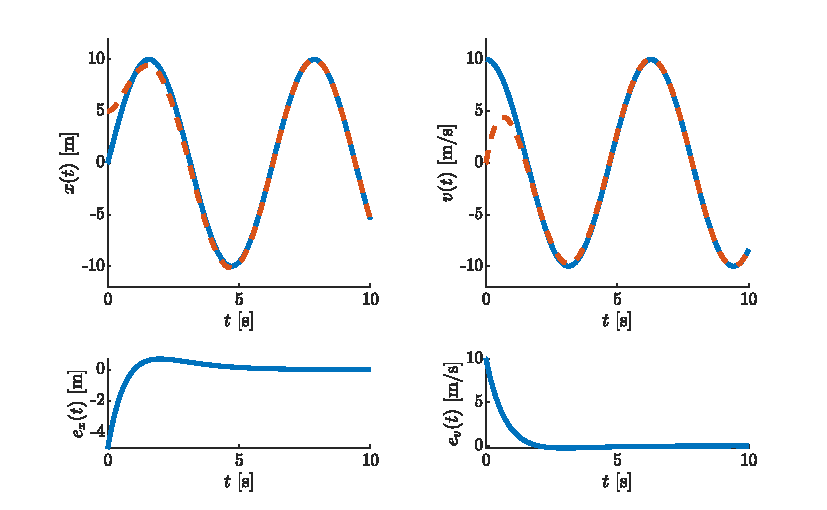
\includegraphics{figures/ex417.pdf}

The solid line is the true state and the dashed line is the estimate from the observer. 

The error dynamics are 
\begin{align*}
    \dot e &= \left(A - K\,C\right)\,e = \left(\begin{pmatrix}
        0 & 1 \\ -\omega_0 & 0
    \end{pmatrix} - \begin{pmatrix}
        k_1 \\ k_2
    \end{pmatrix}\,\begin{pmatrix}
        0 & 1
    \end{pmatrix}\right)\,e = \begin{pmatrix}
        0 & 1 - k_1 \\ -\omega_0^2 & -k_2
    \end{pmatrix}\,e,\\
    \dot e_x &= (1 - k_1)\,e_v \quad \dot e_v = -\omega_0^2\,e_x - k_2\,e_v \quad \implies \dot e_x = e_v \quad \dot e_v = -\omega_0^2\,e_x - 2\,\omega_0\,e_v.
\end{align*}
Therefore, the error will converge with a time constant of $1/\omega_0$.

\clearpage
\subsection*{Code}

\begin{matlabcode}
    clear; 
    
    omega = 1;
    v0 = 10;
    
    % system true states
    x = @(t) 10*sin(omega*t);
    v = @(t) 10*cos(omega*t);
    
    A = [0 1; -omega^2 0];
    C = [0 1];
    
    y0 = [5; 0];
    tspan = [0 10];
    [t,y] = ode45(@(t,y) observ(y,v(t),C,A,omega),tspan, y0);
    
\end{matlabcode}

\matlabheading{functions}
    
\begin{matlabcode}
    function xdot = observ(x,y,C,A,omega)
    
    K = [0; 2*omega];
    
    xdot = A*x + K*(y - C*x);
    
    end
\end{matlabcode}
\clearpage
\section{Kailath 4.1-8}
The model:
\begin{align*}
    \ddot x - 2\omega\dot y - 9\omega^2x &= 0 & \ddot y + 2\omega\dot x + 4\omega^2y &= u.
\end{align*}
Let, 
\begin{align*}
    \dot x &= v_x, \quad \dot y = v_y & \implies \ddot x = \dot v_x, \quad \ddot y &= \dot v_y. 
\end{align*}
Therefore, 
\begin{align*}
    \dot v_x - 2\omega v_y - 9\omega^2x &= 0 & \dot v_y + 2\omega v_x + 4\omega^2y &= u, \\
    \dot v_x &= 2\omega v_y + 9\omega^2x & \dot v_y &= u - 2\omega v_x - 4\omega^2y. \\
\end{align*}
The state matrix, $X = \begin{pmatrix} x & v_x & y & v_y \end{pmatrix}^T$. The system can be re-written as 
\newcommand{\A}{\begin{pmatrix}
    0 & 1 & 0 & 0\\
    9\omega^2 & 0 & 0 & 2\omega \\
    0 & 0 & 0 & 1 \\
    0 & -2\omega & -4\omega^2 & 0 
\end{pmatrix}}
\begin{align*}
    \dot X &= \A\,X + \begin{pmatrix}
        0 \\ 0 \\ 0 \\ 1
    \end{pmatrix}\,u, & y &= \begin{pmatrix}
        0 & 0 & 1 & 0
    \end{pmatrix}\,X.
\end{align*}
The closed-loop observer poles 
\begin{align*}
    \alpha_\mathcal{O}(s) &= \text{det}\left(SI - A + K\,C\right) \\
    &= \text{det}\left(\begin{pmatrix}
        s & 0 & 0 & 0 \\ 0 & s & 0 & 0 \\ 0 & 0 & s & 0 \\ 0 & 0 & 0 & s
    \end{pmatrix} - \A + \begin{pmatrix}
        k_1 \\ k_2 \\ k_3 \\ k_4
    \end{pmatrix}\,\begin{pmatrix}
        0 & 0 & 1 & 0
    \end{pmatrix}\right) \\
    &= \text{det}\begin{pmatrix}
        s & -1 & k_1 & 0 \\ -9\omega^2 & s & k_2 & -2\omega \\ 0 & 0 & k_3 + s & -1 \\ 0 & 2\omega & 4\omega^2 + k_4 & s
    \end{pmatrix}\\
    &= s^4 + k_3s^3 + \left(k_4 - \omega^2\right)s^2 + (-5k_3\omega^2-2k_2\omega)s - 36\omega^4 - 18k_1\omega^3 - 9k_4\omega^2
\end{align*}
The closed-loop observer poles are $s = -2\omega$, $s = -3\omega$, $s = -3\omega \pm j3\omega$
\begin{align*}
    \alpha_\mathcal{O}(s) &= \left(s + 2\omega\right)\,\left(s + 3\omega_0\right)\,\left(s + 3\omega - j3\omega\right)\,\left(s + 3\omega + j3\omega\right) \\
    &= s^4 + 11\omega s^3 + 54\omega^2 s^2 + 126\omega^3 s + 108\omega^4
\end{align*}
Now, 
\begin{align*}
    \begin{array}{rcl}
        k_3 & = & 11\omega \\
        k_4 - \omega^2 & = & 54\omega^2 \\
        5k_3\omega^2 + 2k_2\omega & = & -126\omega^3 \\
        36\omega^4 + 18k_1\omega^3 + 9k_4\omega^2 & = & -108\omega^4
    \end{array} \qquad \implies \begin{array}{rcl}
        k_1 & = & -\frac{71}{2}\omega \\ 
        k_2 & = & -\frac{181}{2}\omega^2 \\
        k_3 & = & 11\omega \\ 
        k_4 & = & 55\omega^2.
    \end{array} 
\end{align*}
The observer is 
\begin{align*}
    \dot{\hat X} &= A\,\hat X + B\,u + K\,\left(y - C\,\hat X\right)
\end{align*}
The simulation results are shown in the figure below, the blue curve is the 'true' state and rthe orange is the estimated from the observer.

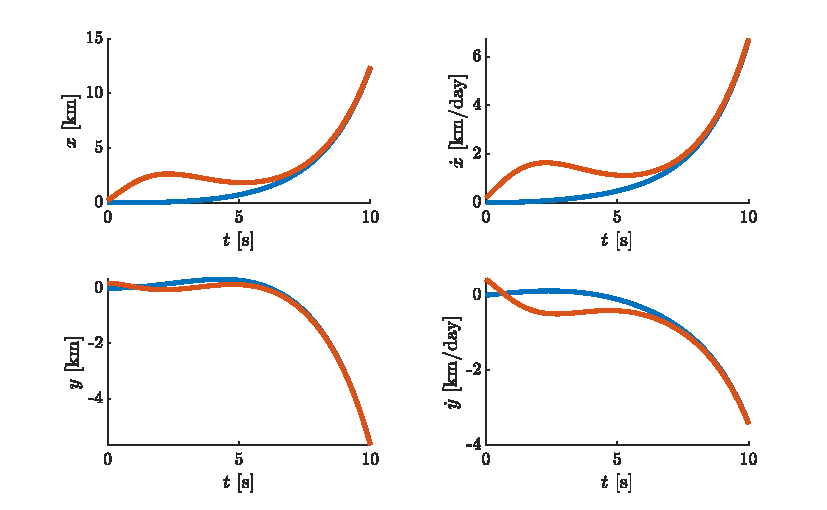
\includegraphics{figures/ex418.pdf}

The error between the estimated states and the 'true' states is shown 

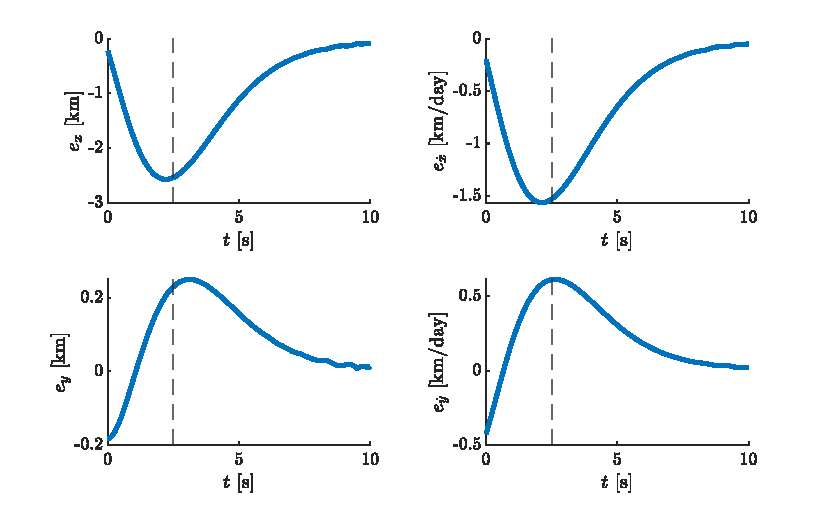
\includegraphics{figures/ex418_err.pdf}

From the figure, it is clear that after 2.5\,days the error starts to decay.

\subsection*{Code}
\matlabheading{Algebra}

\begin{matlabcode}
syms s w
e1 = collect((s + 2*w) * (s + 3*w) * ... 
        ... (s + 3*w + 1j*3*w) * (s + 3*w - 1j*3*w),s);
c1 = coeffs(e1,s); c1(end) = [];
S = s*eye(4);
A = [0, 1, 0, 0;...
     9*w^2, 0, 0, 2*w;...
     0, 0, 0, 1;...
     0, -2*w, -4*w^2, 0]; 
K = sym('k',[4 1]); C = [0 0 1 0];
e2 = collect(det(S - A + K*C),s);
c2 = coeffs(e2,s); c2(end) = [];
eqns = c1 == c2; 
Sol = solve(eqns,K); 
\end{matlabcode}

\matlabheading{system simulation (true-states)}

\begin{matlabcode}
omega = 2*pi/29.3; % orbital frequency [rad/s]
u = 1000 / (300 * omega^2) ; % input (F/(m*w^2)) [m/rad^2]
% state space representation [x; xdot; y; ydot]
A = [0, 1, 0, 0;...
     9*omega^2, 0, 0, 2*omega;...
     0, 0, 0, 1;...
     0, -2*omega, -4*omega^2, 0];
B = [0; 0; 0; 1]; C = [0, 0, 1, 0];
bryson_sattelite = @(t,x) A*x + B*u;

% simulation
y0 = [0; 0; 0; 0]; % initial states
tspan = [0 10]; % [days]
[t, y] = ode45(@(t,y) bryson_sattelite(t,y),tspan,y0);
\end{matlabcode}

\matlabheading{observer}

\begin{matlabcode}
% state observer 
K = [-71/2*omega; -181/2*omega^2; 11*omega; 55*omega^2];
mesh = @(x) interp1(t,y(:,3),x);
obs_bryson_sattelite = @(t,x) A*x + B*u + K*(mesh(t) - C*x);

% simulation 
y0 = rand([4 1]) * 500; % initial states
[to, yo] = ode45(@(t,y) obs_bryson_sattelite(t,y),tspan,y0); 

% error
for ii = 1:width(y)
    yq = interp1(t,y(:,ii),to);
    eq(:,ii) = yq - yo(:,ii);
end
\end{matlabcode}
\clearpage
\section{Kailath 4.1-9}
In discrete time systems, the error at time-step $N$ is 
\begin{align*}
    e_{N} &= \left(A - K\,C\right)\,e_{N-1}
\end{align*}
The error $e_N = 0$, at time-step $N$ ig $K$ is the eigen-values of $\left(A - K\,C\right)$.

\clearpage
\section{Kailath 4.3-4}
The state-space model of the inertial navigator is 
\begin{align*}
    \begin{pmatrix}
        \dot v \\ \dot \varphi \\ \dot \varepsilon
    \end{pmatrix} &= \begin{pmatrix}
        0 & -1 & 0 \\ 1 & 0 & 1 \\ 0 & 0 & 0
    \end{pmatrix}\,\begin{pmatrix}
        v \\ \varphi \\ \varepsilon
    \end{pmatrix} + \begin{pmatrix}
        0 \\ 0 \\ w
    \end{pmatrix}
\end{align*}
(a) Determining the solutions. 
\begin{align*}
    X(s) = 0 \quad \det{\left(sI - A\right)} &= 0 \\
    \det\begin{pmatrix}
        s & 1 & 0 \\ -1 & s & -1 \\ 0 & 0 & s
    \end{pmatrix} &= 0\\
    s\,\left(s^2 + 1\right) &= 0.
\end{align*}
The open-loop eigen values are $\lambda_1 = 0$, $\lambda_{2,3} = \pm j$

(b) observer design 
\begin{align*}
    y = \begin{pmatrix}
        1 & 0 & 0
    \end{pmatrix}\,\begin{pmatrix}
        v \\ \varphi \\ \varepsilon 
    \end{pmatrix}
\end{align*}
The observer is 
\begin{align*}
    \dot{\hat X} &= A\,\hat X + B\,u + K\,\left(y - C\,\hat X\right) \\
    \begin{pmatrix}
        \dot{\hat v} \\ \dot{\hat \varphi} \\ \dot{\hat \varepsilon}
    \end{pmatrix} &= \begin{pmatrix}
        0 & -1 & 0 \\ 1 & 0 & 1 \\ 0 & 0 & 0
    \end{pmatrix}\,\begin{pmatrix}
        \hat v \\ \hat \varphi \\ \hat \varepsilon
    \end{pmatrix} + \begin{pmatrix}
        0 \\ 0 \\ w
    \end{pmatrix} + K\,\left(y - \begin{pmatrix}
        1 & 0 & 0
    \end{pmatrix}\,\begin{pmatrix}
        \hat v \\ \hat \varphi \\ \hat \varepsilon
    \end{pmatrix}\right)
\end{align*}
The closed-loop observer poles 
\begin{align*}
    \alpha_\mathcal{O}(s) &= \text{det}\left(SI - A + K\,C\right) \\
    &=  \det\left(\begin{pmatrix}
        s & 0 & 0 \\ 0 & s & 0 \\ 0 & 0 & s
    \end{pmatrix} - \begin{pmatrix}
        0 & -1 & 0 \\ 1 & 0 & 1 \\ 0 & 0 & 0
    \end{pmatrix} + \begin{pmatrix}
        k_1 \\ k_2 \\ k_3 
    \end{pmatrix}\,\begin{pmatrix}
        1 & 0 & 0
    \end{pmatrix}\right)\\
    &= \det\begin{pmatrix}
        k_1 + s & 1 & 0 \\ k_2 - 1 &  s -1 \\ k_3 & 0 & s
    \end{pmatrix} \\
    &= s^3 + k_1\,s^2 + \left(1 - k_2\right)\,s - k_3
\end{align*}
The closed-loop observer poles are $s = -10$, $s = -0.1$, $s = -0.1$
\begin{align*}
    \alpha_\mathcal{O}(s) &= \left(s + 10\right)\,\left(s + 0.1\right)\,\left(s + 0.1\right) \\
    &= s^3 + 10.2\,s^2 + 2.01\,s + 0.1
\end{align*}
The gains are 
\begin{align*}
    K = \begin{pmatrix}
        k_1 & k_2 & k_3
    \end{pmatrix}^T = \begin{pmatrix}
        10.2 & -1.01 & -0.1
    \end{pmatrix}^T
\end{align*}
The simulation results of the observer is shown in the next page
\clearpage

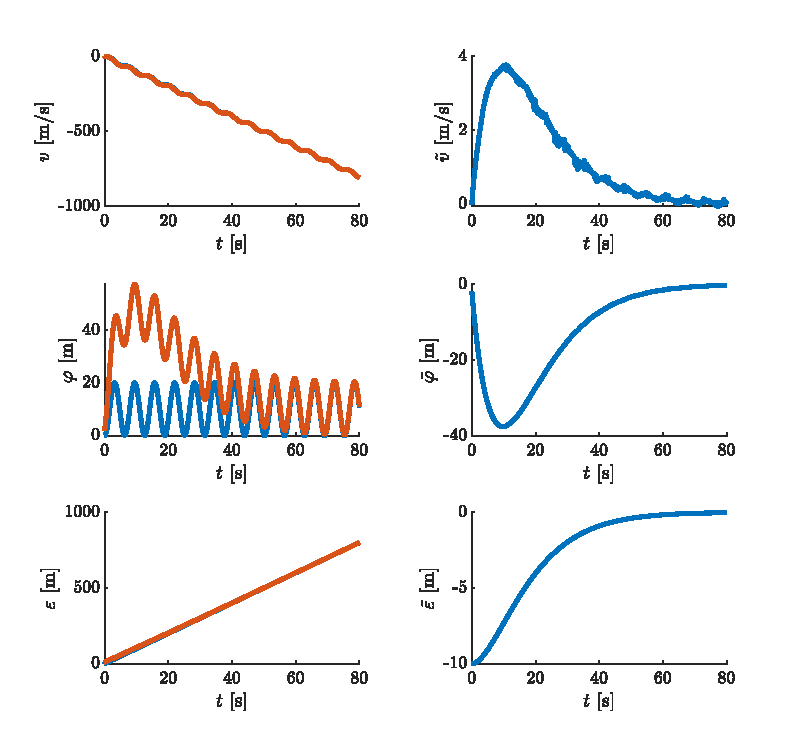
\includegraphics{figures/le4_3_7a.pdf}

The estimated states from the observer are shown in orange and the 'true' states are shown in blue.

(c) The \emph{second order} observer. 
Original state equations
\begin{align*}
    \begin{pmatrix}
        \dot v \\ \dot \varphi \\ \dot \varepsilon
    \end{pmatrix} &= \begin{pmatrix}
        0 & -1 & 0 \\ 1 & 0 & 1 \\ 0 & 0 & 0
    \end{pmatrix}\,\begin{pmatrix}
        v \\ \varphi \\ \varepsilon
    \end{pmatrix} + \begin{pmatrix}
        0 \\ 0 \\ w
    \end{pmatrix}, &  
    \text{or } \begin{pmatrix}
        \dot \varepsilon \\ \dot \varphi \\ \dot v 
    \end{pmatrix} &= \begin{pmatrix}
        0 & 0 & 0 \\ 1 & 0 & 1 \\ 0 & -1 & 0
    \end{pmatrix}\,\begin{pmatrix}
        \varepsilon \\ \varphi \\ v
    \end{pmatrix} + \begin{pmatrix}
        w \\ 0 \\ 0
    \end{pmatrix}
\end{align*}
Considering partitioned state equations 
\begin{align*}
    \begin{pmatrix}
        \dot x_r \\ \dot x_n 
    \end{pmatrix} &= \begin{pmatrix}
        A_r & a_r \\ a_n & a_{nn} 
    \end{pmatrix}\,\begin{pmatrix}
        x_r \\ x_n 
    \end{pmatrix} + \begin{pmatrix}
        b_r \\ b_n 
    \end{pmatrix}\,u(t) & y &= x_n \\
    \begin{pmatrix}
        \begin{pmatrix} \dot{\hat \varepsilon} \\ \dot{\hat \varphi} \end{pmatrix} \\ \dot{\hat v} 
    \end{pmatrix} &= \begin{pmatrix}
        \begin{pmatrix}
            0 & 0 \\ 1 & 0
        \end{pmatrix} & \begin{pmatrix}
            0 \\ 1
        \end{pmatrix} \\
        \begin{pmatrix}
            0 & -1
        \end{pmatrix} & 0
    \end{pmatrix}\,\begin{pmatrix}
        \begin{pmatrix} \hat \varepsilon \\ \hat \varphi \end{pmatrix} \\ \hat v
    \end{pmatrix} + \begin{pmatrix}
        \begin{pmatrix} w \\ 0 \end{pmatrix} \\ 0
    \end{pmatrix} & y &= v
\end{align*} 

\fbox{\parbox{0.95\textwidth}{
    Change in partitioning affects the pole placement of the reduced order observer, with $\begin{pmatrix}
        \begin{pmatrix}
            \varphi & \varepsilon
        \end{pmatrix} & v
    \end{pmatrix}^T$, only one pole (of the reduced order observer) can be placed arbitrarily.
}}

The closed-loop poles 
\begin{align*}
    \alpha_\mathcal{O}(s) &= \det\left(sI - A_r + L\,a_n\right) \\
    &= \det\left(\begin{pmatrix}
        s & 0 \\ 0 & s
    \end{pmatrix} - \begin{pmatrix} 0 & 0 \\ 1 & 0 \end{pmatrix} + \begin{pmatrix}
        l_1 \\ l_2
    \end{pmatrix}\,\begin{pmatrix} 0 & -1 \end{pmatrix}\right) \\
    &= \det\left(\begin{pmatrix}
        s-1 & -l_1 \\ -1 & s-l_2
    \end{pmatrix}\right) = s^2 -l_2\,s - l_1
\end{align*}

The closed-loop observer poles are $s = -0.1$, $s = -0.1$
\begin{align*}
    \alpha_\mathcal{O}(s) &= \left(s + 0.1\right)\,\left(s + 0.1\right) = s^2 + 0.2\,s + 0.01
\end{align*}

The gains are 
\begin{align*}
    L = \begin{pmatrix}
        l_1 & l_2 
    \end{pmatrix}^T = \begin{pmatrix}
        -0.01 & -0.2
    \end{pmatrix}^T
\end{align*}

The observer is designed as, 
\begin{align*}
    \dot{\hat \theta} &= \left(A_r - L\,a_n\right)\,\theta + \left(a_r - L\,a_{nn} + A_r\,L - L\,a_n\,L\right)\,y + (b_r - b_n)\,u \\
    \hat x_r &= \theta + L\,y \\
    \hat x_n &= x_n = y
\end{align*}
% The closed-loop poles (altered partioning)
% \begin{align*}
%     \alpha_\mathcal{O}(s) &= \det\left(sI - A_r + L\,a_n\right) \\
%     &= \det\left(\begin{pmatrix}
%         s & 0 \\ 0 & s
%     \end{pmatrix} - \begin{pmatrix} 1 & 0 \\ 0 & 0 \end{pmatrix} + \begin{pmatrix}
%         l_1 \\ l_2
%     \end{pmatrix}\,\begin{pmatrix} 0 & -1 \end{pmatrix}\right) \\
%     &= \det\left(\begin{pmatrix}
%         s-1 & -l_1 \\ 0 & s-l_2
%     \end{pmatrix}\right) = \left(s - 1\right)\,\left(s - l_2\right)
% \end{align*}
% Placing the estimator poles at $-0.1$, gives $l_2 = -0.1$.

The simulation results of the observer are shown below, where the estimated states from the observer are shown in orange, and the 'true' states are shown in blue.

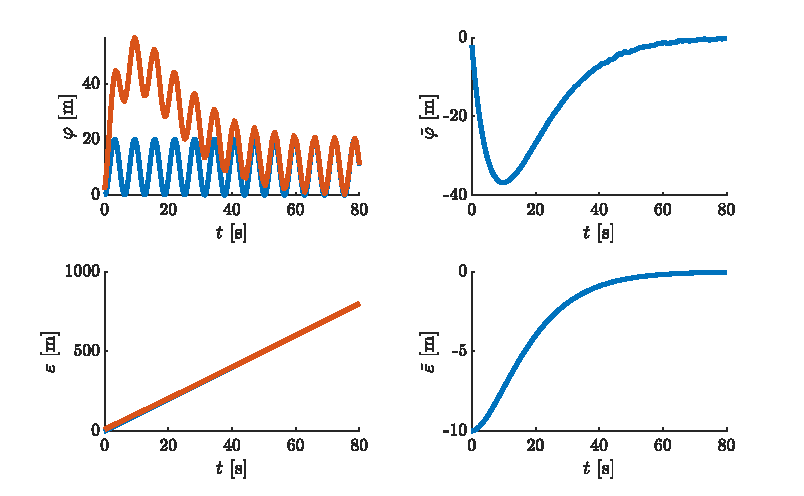
\includegraphics{figures/le4_3_7b.pdf}

\fbox{\parbox{0.95\textwidth}{
    The reduced-order and the full-order observer are similar in performance.
}}

\section*{Code}
\matlabheading{simulation (true system)}

\begin{matlabcode}
clear;
u = 10;
A = [0 -1 0; 1 0 1; 0 0 0];
B = [0; 0; 1]; C = [1 0 0];
int_nav = @(t,x) A*x + B*u;

% simulation
y0 = [0; 0; 0]; % initial states
tspan = [0 80]; % [s]
[t, y] = ode45(@(t,y) int_nav(t,y),tspan,y0);
\end{matlabcode}


\matlabheading{Observer simulation}

\begin{matlabcode}
% state observer 
K = [10.2; -1.01; -0.1];
mesh = @(x) interp1(t,y(:,1),x,'spline');
obs_int_nav = @(t,x) A*x + B*u + K*(mesh(t) - C*x);

% simulation 
y0 = [0; 2; 10]; % initial states
[to, yo] = ode45(@(t,y) obs_int_nav(t,y),tspan,y0); 

% error
for ii = 1:width(y)
    yq = interp1(t,y(:,ii),to);
    eq(:,ii) = yq - yo(:,ii);
end
\end{matlabcode}


\matlabheading{Reduced order observer simulation}

\begin{matlabcode}
% A-matrix partition
Ar = [0 0; 1 0];
cr = [0 -1];
br = [0; 1];
ann = 0;
% B_matrix
gr = [1; 0];
gn = 0;
% observer gain
L = [-0.01; -0.2];
% state observer
red_obs_int_nav = @(t,z) (Ar - L*cr)*z ... 
                  + (br -L*ann + Ar*L - L*cr*L)*mesh(t) ...
                  + (gr - L*gn)*u;

% simulation
y0 = [10; 2]; % initial states
[tr, zo] = ode45(@(t,y) red_obs_int_nav(t,y),tspan,y0); 

% states
for ii = 1:length(tr)
    xr(ii,:) = zo(ii,:) + (L*mesh(tr(ii)))';
end

% error
yq = interp1(t,y(:,3),tr);
eq2(:,1) = yq - xr(:,1);
yq = interp1(t,y(:,2),tr);
eq2(:,2) = yq - xr(:,2);
\end{matlabcode}
\clearpage

\chapter{Observers for DAEs and non-Linear Systems}
\section{Le 2.1}

Consider the following DAE:
\begin{align*}
    E\,\dot x &= A\,x + B\,u, & y &= C\,x
\end{align*}
There exists invertible matrices $P$ and $T$, where $x = T\,w$ and multiplying the model equations with $P$ from the left and $T,$ $T^{-1}$ to the right of $E$ gives 
\begin{align*}
    P\,E\,T\,T^{-1}\dot x &= P\,A\,T\,T^{-1}\,x + P\,B\,T\,T^{-1}\,u. \\
    P\,E\,T\,\dot w &= P\,A\,T\,w + P\,B\,T\,T^{-1}\,u,
\end{align*}
where
\begin{align*}
    P\,E\,T = \begin{pmatrix}
        I & 0 \\ 0 & E_2 
    \end{pmatrix} \quad P\,A\,T = \begin{pmatrix}
        A_1 & 0 \\ 0 & I
    \end{pmatrix}, \quad \text{where $E_2$ is nilpotent.}
\end{align*}
% Note that $P\,E\,T \equiv E$, and $P\,A\,T \equiv A$.

Assuming that the ODE part, $\dot w_1 = A_1\,w_1 + B_1\,u$ is observable, i.e., 
\begin{align*}
    \begin{pmatrix}
        \lambda\,I - A_1 \\ C
    \end{pmatrix} \quad \text{has full column rank } \forall \lambda, \text{ i.e., } \begin{pmatrix}
        \lambda\,I - A_1 \\ 0 \\ C
    \end{pmatrix} \text{ also has full column rank } \forall \lambda.
\end{align*}

Considering the following:
\begin{align*}
    \begin{pmatrix}
        \lambda\,E - A \\ C
    \end{pmatrix} &\equiv \begin{pmatrix}
        \lambda\,P\,E\,T - P\,A\,T \\ C
    \end{pmatrix} = \begin{pmatrix}
        \lambda\,\begin{pmatrix}
            I & 0 \\ 0 & E_2 
        \end{pmatrix} - \begin{pmatrix}
            A_1 & 0 \\ 0 & E_2 
        \end{pmatrix} \\ \begin{pmatrix}
            C_1 & C_2
        \end{pmatrix}
    \end{pmatrix}
    = \begin{pmatrix}
        \lambda\,I - A_1 & 0 \\ 0 & \lambda\,E_2 - I \\ C_1 & C_2
    \end{pmatrix}
\end{align*}
Any square matrix has a Jordan normal form if the field of coefficients is extended to one containing all the eigenvalues of the matrix [\emph{from Wikipedia}].
The Jordan form is given as 
\begin{align*}
    \begin{pmatrix}
        \lambda_1 & 1 \\ & \lambda_1 & 1 \\ & & \lambda_1 \\ & & & \lambda_2 & 1 \\ & & & & \lambda_2 \\ & & & & & \lambda_3 \\ & & & & & & \ddots \\ & & & & & & & \lambda_n 
    \end{pmatrix}, \text{for a nilpotent matrix}, \lambda_1 = \lambda_2 = \cdots = \lambda_n = 0
\end{align*}
Thus, $\lambda\,E_2 - I$ has always full-column rank. 

\fbox{
    \parbox{0.95\textwidth}{
        Therefore, if $\begin{pmatrix}
            \lambda\,I - A_1 & C
        \end{pmatrix}^T$ has full-column rank then $\begin{pmatrix}
            \lambda\,E - A & C
        \end{pmatrix}^T$ has full-column rank $\forall\ \lambda$. \\
        
        If $\begin{pmatrix}
            \lambda\,E - A & C
        \end{pmatrix}^T$ has full-column rank then its minor $\begin{pmatrix}
            \lambda\,I - A_1 & C
        \end{pmatrix}^T$ also has full-column rank $\forall\ \lambda$.
    }
}


% The DAE can be partitioned as
% \begin{align*}
%     E_1\,\dot x_1 &= A_1\,x_1 + B_1\,u, & E_2\,\dot x_2 &= A_2\,x_2 + B_2\,u, & y &= \begin{pmatrix}
%         C_1 & C_2
%     \end{pmatrix}\,x
% \end{align*}
% with $E_2\,\dot x_2 = A_2\,x_2 + B_2\,u,$ beging the ODE, i.e., usually $E_2 = I$.
% \begin{align*}
%     \begin{pmatrix}
%         E_1 & 0 \\ 0 & E_2
%     \end{pmatrix}\,\dot x &= \begin{pmatrix}
%         A_1 & 0 \\ 0 & A_2
%     \end{pmatrix}\,x + \begin{pmatrix}
%         B_1 \\ B_2
%     \end{pmatrix}\,u & y &= \begin{pmatrix}
%         C_1 & C_2
%     \end{pmatrix}\,x
% \end{align*}

% Assume that the ODE part of the system is observable, i.e.,
% \begin{align*}
%     \text{rank}\begin{pmatrix}
%         \lambda E_1 - A_1 \\ C_1
%     \end{pmatrix} = n
% \end{align*}

% The observability matrix for the entire system can be written as
% \begin{align*}
%     \mathcal{O}x &= \begin{pmatrix}
%         \lambda \begin{pmatrix}
%             E_1 & 0 \\ 0 & E_2
%         \end{pmatrix} - \begin{pmatrix}
%             A_1 & 0 \\ 0 & A_2
%         \end{pmatrix} \\ \begin{pmatrix}
%             C_1 & C_2
%         \end{pmatrix}
%     \end{pmatrix}
%     = \begin{pmatrix}
%         \lambda E_1 - A_1 & 0 \\ 0 & \lambda E_2 - A_2 \\ C_1 & C_2
%     \end{pmatrix}
% \end{align*}
% \begin{theorem}
%     If $A$ is an $n \times m$ matrix, then the determinant of a $p \times p$ submatrix obtained from $A$ is called a minor of order $p$.
% \end{theorem}

% The submatrix is $\begin{pmatrix}
%     \lambda E_1 - A_1
% \end{pmatrix}$ and has the order $p$, with $p$ number of 'states'. Since this is an ODE, this matrix is non-zero

% The submatrix is $\begin{pmatrix}
%     \lambda E_2 - A_2
% \end{pmatrix}$ and has the order $q$, with $q$ number of 'states'. Since this is part of a DAE this has the set of algebraic expressions which is also not a non-zero matrix.

% For a SISO system, $C_1$ and $C_2$ is not a square matrix.

% % The largest minor is $\begin{pmatrix}
% %     \lambda E_2 - A_2 \\ C_2
% % \end{pmatrix}$.

% % $\det\begin{pmatrix}
% %     \lambda E_2 - A_2
% % \end{pmatrix}$ is non-zero since the ODE is observable.

% \begin{theorem}
%     The rank of an $n \times m$ matrix is equal to the order of its largest non-zero minor.
% \end{theorem}

% % The rank of $\det\begin{pmatrix}
% %     \lambda E_2 - A_2 \\ C_2
% % \end{pmatrix}$ is the equal to the order of $\det\begin{pmatrix}
% %     \lambda E_2 - A_2
% % \end{pmatrix}$, which is equal to the number of states $n$.

% \begin{theorem}
%     A tall $n \times m$ matrix is full column is \underline{if and only if} there exists a non-zero minor of order $p$.
% \end{theorem}

% % Therefore,...
% 1
\clearpage 
\section{Le 2.2}
(a) Writing the model equations in the form 
\begin{align*}
    E\,\dot x &= A\,x + B\,u
\end{align*}

The model equations are
\begin{align*}
    u - v_1 &= R_1\,i_1 & 
    v_3 - v_4 &= R_2\,i_2 & 
    v_1 - v_4 &= R_3\,i_3 & 
    C\,\dot v_1 -C\,\dot v_3 &= i_2 \\
    v_1 - v_2 &= 0 & 
    v_2 &= 0 & 
    i_1 &= i_2 + i_3 \\
    v_1 + R_1\,i_1 &= u & 
    v_3 - v_4 - R_2\,i_2 &= 0 & 
    v_1 - v_4 - R_3\,i_3 &=  0& 
    C\,\dot v_1 -C\,\dot v_3 - i_2 &= 0\\
    v_1 - v_2 &= 0 & 
    v_2 &= 0 & 
    i_1 - i_2 - i_3 &= 0
\end{align*}

Considering $x = \begin{pmatrix} i_1 & i_2 & i_3 & v_1 & v_2 & v_3 & v_4 \end{pmatrix}^T$,
\begin{align*}
    \begin{pmatrix}
        %   i1  & i2    & i3    & v1    & v2    & v3    & v4     
            0   & 0     & 0     & 0     & 0     & 0     & 0 \\
            0   & 0     & 0     & 0     & 0     & 0     & 0 \\
            0   & 0     & 0     & 0     & 0     & 0     & 0  \\
            0   & 0     & 0     & C_c   & 0     & -C_c  & 0 \\
            0   & 0     & 0     & 0     & 0     & 0     & 0  \\
            0   & 0     & 0     & 0     & 0     & 0     & 0  \\
            0   & 0     & 0     & 0     & 0     & 0     & 0 
        \end{pmatrix}\,\begin{pmatrix} 
            \dot i_1 \\ \dot i_2 \\ \dot i_3 \\ \dot v_1 \\ \dot v_2 \\ \dot v_3 \\ \dot v_4
        \end{pmatrix} &= \begin{pmatrix}
    %   i1    & i2  & i3    & v1    & v2    & v3    & v4    
        -R_1& 0     & 0     & -1    & 0     & 0     & 0 \\
        0   & -R_2  & 0     & 0     & 0     & 1     & -1 \\
        0   & 0     & -R_3  & 1     & 0     & 0     & -1 \\
        0   & 1     & 0     & 0     & 0     & 0     & 0 \\
        0   & 0     & 0     & 1     & -1    & 0     & 0\\
        0   & 0     & 0     & 0     & 1     & 0     & 0\\
        1   & -1    & -1    & 0     & 0     & 0     & 0
    \end{pmatrix}\,\begin{pmatrix} 
        i_1 \\ i_2 \\ i_3 \\ v_1 \\ v_2 \\ v_3 \\ v_4 
    \end{pmatrix} \\ 
    & \qquad + \begin{pmatrix} 1 \\ 0 \\ 0 \\ 0 \\ 0 \\ 0 \\ 0 \end{pmatrix}\,u
\end{align*}

(b) Measurement signals: 

Choosing $C$ such that $\begin{pmatrix}
    \lambda\,E - A & C
\end{pmatrix}^T$ has full-rank $\forall\ \lambda$. 

$\lambda\,E - A$ is 0, when $\det\left(\lambda\,E - A\right) = 0$, i.e., $\lambda = \frac{-1}{C_c\,\left(R_2 + R_3\right)}$ 

The matrix $\begin{pmatrix}
    \lambda\,E - A & C
\end{pmatrix}^T$ \underline{does not} have full-rank with the measurement signals $\begin{Bmatrix}
    i_1, v_1, v_2
\end{Bmatrix}\ \forall\ \lambda$.

% \underline{Alternative:}
% The algebraic expressions can be determined using the input so considering the ODE
% \begin{align*}
%     C_c\,\dot v_1 -C_c\,\dot v_3 - i_2 &= 0 & \&\ v_1 - v_2 &= 0, \quad
%     v_2 = 0 \\
%     & & \implies \dot v_1 - \dot v_2 &= 0, \quad
%     \dot v_2 = 0 \\
%     & & \implies \dot v_1 &= 0,
% \end{align*}
% Therefore, $C_c\,\dot v_1 -C_c\,\dot v_3 - i_2 = 0$ reduces to $ C_c\,\dot v_3 = i_2 $

% To estimate the state $v_3$, $i_2$ is needed and $i_2$ can be determined by the following:
% \begin{align*}
%     i_2 &= i_1 - i_3, & i_2 &= \frac{u - v_1}{R_1} - i_3, & i_2 &= \frac{u - v_1}{R_1} - \frac{v_1 - v_4}{R_3}\\
%     i_2 &= \frac{v_3 - v_4}{R_2}, & \implies  R_2\,C_c\,\dot v_3 &= v_3 - v_4
% \end{align*}
% % The following are the possible measurement equations
% % \begin{align*}
% %     y &= \begin{cases}
% %         v_3 \\
% %         i_2 \\
% %         i_3 \\
% %         v_4 \\
% %         \begin{pmatrix}
% %             1 & -1
% %         \end{pmatrix}\,\begin{pmatrix}
% %             i_1 & i_3 
% %         \end{pmatrix} \\
% %         \begin{pmatrix}
% %             1 & 0 \\ 0 & 1
% %         \end{pmatrix}\,\begin{pmatrix}
% %             i_1 & i_3 
% %         \end{pmatrix} 
% %     \end{cases} & \text{The single measurements that does not work}\ \begin{Bmatrix}
% %         i_1, v_1, v_2
% %     \end{Bmatrix}
% % \end{align*}

% The single measurements that do not work $\begin{Bmatrix}
%         i_1, v_1, v_2
%     \end{Bmatrix}$1

(c) Building an observer 

Simplifying the ODE, 
\begin{align*}
    C\,\dot v_1 -C\,\dot v_3 - i_2 &= 0 & \implies C\,\dot v_3 &= \frac{v_3 - v_4}{R_2}.\\
\end{align*}
The measurement equation:
\begin{align*}
    y = v_4.
\end{align*}
The observer design is 
\begin{align*}
    \dot{\hat v}_3 = \frac{\hat v_3 - v_4}{R_2\,C_c} + K\,\left(v_4 - 0\right)
\end{align*}

The poles for the observer is 
\begin{align*}
    \alpha_\mathcal{O}(s) &= \det\left(s\,I - A + K\,C\right) \\
    &= s - \frac{1}{R_2\,C_c} + k_1\times 0.
\end{align*}

% Assuming that $R_1 = R_2 = R_3 = R$.
% 
% The poles for the observer is 
% \begin{align*}
%     \alpha_\mathcal{O}(s) &= \det\left(s\,E - A + K\,C\right) \\
%     &= \left(2\,C_{c}\,R^2-C_{c}\,R^2\,k_{1}+C_{c}\,R^2\,k_{2}+C_{c}\,R^2\,k_{3}-3\,C_{c}\,R^2\,k_{5}-3\,C_{c}\,R^2\,k_{6}-C_{c}\,R^3\,k_{7}\right)\,s \\
%     &\quad + R-R\,k_{1}+R\,k_{3}-2\,R\,k_{5}-2\,R\,k_{6}-R^2\,k_{4}-R^2\,k_{7}
% \end{align*}
% 
% Considering the following partitioned DAE, 
% \begin{align*}
%     \begin{pmatrix}
%         0   & 0     & 0     & C_c   & 0     & -C_c  & 0 
%     \end{pmatrix}\,\dot X &= \begin{pmatrix}
%         0   & 1     & 0     & 0     & 0     & 0     & 0 
%     \end{pmatrix}\,X
%     \\
%     \begin{pmatrix}
%         %   i1  & i2    & i3    & v1    & v2    & v3    & v4     
%             0   & 0     & 0     & 0     & 0     & 0     & 0 \\
%             0   & 0     & 0     & 0     & 0     & 0     & 0 \\
%             0   & 0     & 0     & 0     & 0     & 0     & 0  \\
%             0   & 0     & 0     & 0     & 0     & 0     & 0  \\
%             0   & 0     & 0     & 0     & 0     & 0     & 0  \\
%             0   & 0     & 0     & 0     & 0     & 0     & 0 
%         \end{pmatrix}\,\dot X &= \begin{pmatrix}
%     %   i1    & i2  & i3    & v1    & v2    & v3    & v4    
%         -R_1& 0     & 0     & -1    & 0     & 0     & 0 \\
%         0   & -R_2  & 0     & 0     & 0     & 1     & -1 \\
%         0   & 0     & -R_3  & 1     & 0     & 0     & -1 \\
%         0   & 0     & 0     & 1     & -1    & 0     & 0\\
%         0   & 0     & 0     & 0     & 1     & 0     & 0\\
%         1   & -1    & -1    & 0     & 0     & 0     & 0
%     \end{pmatrix}\,X + \begin{pmatrix} 1 \\ 0 \\ 0 \\ 0 \\ 0 \\ 0 \end{pmatrix}\,u
% \end{align*}
% The ODE part of the model with the measurements is 
% \begin{align*}
%     C_c\,\dot v_1 - C_c\,\dot v_3 = i_2 \text{ reduces to } \dot v_3 = \frac{v_4 - v_3}{R_2\,C_c}, \text{ since } v_1 = v_2 = 0, \qquad y = v_4
% \end{align*}
% % reduces to 
% % \begin{align*}
% %     \begin{pmatrix}
% %         0   & 0     & 0     & 0     & 0     & 1     & 0 
% %     \end{pmatrix}\,\dot X &= \frac{-1}{R_2\,C_c}\begin{pmatrix}
% %         0   & 0     & 0     & 0     & 0     & 1     & -1 
% %     \end{pmatrix}\,X & \text{i.e.,}\ & \dot v_3 = \frac{-1}{R_2\,C_c}\,\left(v_3 - v_4\right)\\ 
% %     y &= \begin{pmatrix}
% %         0   & 0     & 0     & 0     & 0     & 0     & 1
% %     \end{pmatrix}\,X & & y = v_4
% % \end{align*}
% The observer for estimating $\hat v_3$ is 
% \begin{align*}
%     \dot{\hat{v}}_3 &= \frac{1}{R_2\,C_c}\,\left(\hat v_4 - \hat v_3\right)  + K\,\cancelto{0}{\left(y - \hat v_4\right)}
% \end{align*}
% The observer will have the poles at $\frac{-1}{R_2\,C_c}$

% The other 'states' in the system can be determined as 
% \begin{align*}
%     \hat v_2 &= 0 & 
%     \hat v_1 &= \hat v_2 & 
%     \hat i_1 &= \frac{u - \hat v_1}{R_1}, & \\
%     \hat i_2 &= \frac{\hat v_3 - \hat v_4}{R_2}, & 
%     \hat i_3 &= {\hat v_1 - \hat v_4}{R_3}, & 
% \end{align*}

\clearpage
\section{Le 2.3}
The system is defined as 
\begin{align*}
    \dot x &= 1 & y = h(x)
\end{align*}

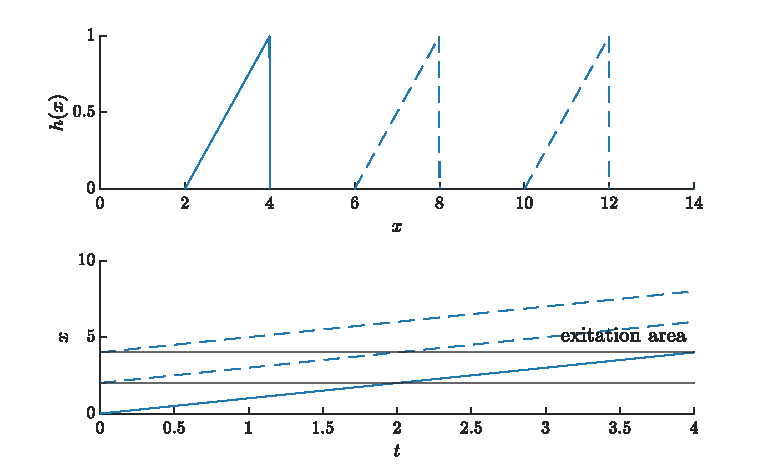
\includegraphics{figures/ex2_3.pdf}

(a) $\mathcal{M} \subset \left(0, 4\right)$ \hspace{4em} \textbf{Weakly observable}. 

\fbox{\parbox{0.98\textwidth}{
    At $x < 2$, $h(x) = 0$ and thus not locally observable. However, $\forall t>=2,\, h(x) = k\,x$ and becomes observable.
}}
% \begin{tabular}{c|c|c}
%      & $\mathcal{M} = \left(0, 4\right)$ & \\
%     \hline
%     locally observable & \textbf{No} & not obs. at $x < 2$, $h(x) = 0$\\ 
%     weakly observable & \textbf{Yes} & obs. at $x \approx 2$, $h(x) = 0$ \\
%     locally weakly observable & \textbf{No} 
% \end{tabular}

(b) $\mathcal{M} = \left(2, 4\right)$ \hspace{4em} \textbf{Locally observable}. 

\fbox{\parbox{0.98\textwidth}{
    $x$ is uniquly isolable for all $\mathcal{U} \subset \mathcal{M}$.
}}

% \begin{tabular}{c|c|c}
%     & $\mathcal{M} = \left(2, 4\right)$ & \\
%    \hline
%    locally observable & \textbf{Yes} & \\ 
%    weakly observable & \textbf{Yes} & \\
%    locally weakly observable & \textbf{Yes} 
% \end{tabular}

(c) $\mathcal{M} = \mathcal{R}^+\ '\cdots'$ \hspace{4em} \textbf{Weakly observable}. 
% \begin{tabular}{c|c|c}
%     & $\mathcal{M} = \mathcal{R}^+\ '\cdots'$ & \\
%    \hline
%    locally observable & \textbf{No} & not obs. at $x < 2\cdots$, $h(x) = 0$\\ 
%    weakly observable & \textbf{Yes} & no unique solutions even for $x < 2$, indistinguishable\\
%    locally weakly observable & \textbf{No} 
% \end{tabular}
% It is still observable in some space [0,2]

\fbox{\parbox{0.98\textwidth}{
    $ 2 \leq t \leq 4,\, h(x) = k\,x$ and becomes observable.
}}

Note:

\fbox{\parbox{0.98\textwidth}{
    if $h(x)$ is a sawtooth waveform, then the system is \textbf{locally weakly observable}.
}}
\clearpage
\section{Le 2.4}
Considering the ODE
\begin{align*}
    \dot x &= 1 & y &= x^3
\end{align*}
Let, 
\begin{align*}
    F(x) &= \begin{pmatrix}
        h(x) \\ L_fh(x) \\ \vdots \\ L_f^qh(x)
    \end{pmatrix} = \begin{pmatrix}
        x^3 \\ 3x^2 \\ 6x \\ \vdots 
    \end{pmatrix}
\end{align*}
The system is indeed locally weakly observable. 1
% The locally weakly observable at $x = 0$ is 
% \begin{align*}
%     \frac{\partial}{\partial x}F(x)\Big|_{x = 0} &= \frac{\partial}{\partial x}\begin{pmatrix}
%         h(x) \\ L_fh(x) \\ L_f^2h(x)
%     \end{pmatrix}_{x = 0} = \begin{pmatrix}
%         3x^2 \\ 6x \\ 6
%     \end{pmatrix}_{x = 0} = \begin{pmatrix}
%         0 \\ 0 \\ 6
%     \end{pmatrix} \text{ is full-rank}
% \end{align*}
% $\frac{\partial}{\partial x}F(x)\Big|_{x = 0}$ is full-rank when $q = 2$, clearly $q > n$.

Considering the ODE
\begin{align*}
    \dot x &= 1 & y &= x\,e^{-1/x^2}
\end{align*}
\begin{align*}
    F(x) &= \begin{pmatrix}
        h(x) \\ L_fh(x) \\ \vdots \\ L_f^qh(x)
    \end{pmatrix} = \begin{pmatrix}
        x\,e^{-1/x^2} \\ \vdots 
    \end{pmatrix}
\end{align*}
Since $x\,e^{-1/x^2}|_{x = 0}$ is $\div 0$. Therefore the locally weakly observable at $x = 0$ is defined as 
\begin{align*}
    \lim_{x \to 0} \frac{\partial}{\partial x}F(x) &= \lim_{x \to 0} \frac{\partial}{\partial x}\begin{pmatrix}
        h(x) 
    \end{pmatrix} \\ 
    &= \lim_{x \to 0} \begin{pmatrix}
        x\,\lambda + \frac{2\,\lambda}{x^2} \\
        \frac{4\,\lambda}{x^5} - \frac{2\,\lambda}{x^3} \\
        \frac{6\,\lambda}{x^4} - \frac{24\,\lambda}{x^6} + \frac{8\,\lambda}{x^8} \\
        \vdots 
    \end{pmatrix} \\
    &= \begin{pmatrix}
        0 \\ 0 \\ 0 \\ \vdots 
    \end{pmatrix},
\end{align*}
where $\lambda = e^{-1/x^2}$

In this case, even as $q \to \infty$, the matrix is not full-rank as $x \to 0$. However, the system is locally weakly observable.

\fbox{
    \parbox{0.95\textwidth}{
        Even if $q$ is $\infty$, it does not imply that the system is not observable. 
    }
}

\subsection*{Code}
\begin{matlabcode}
syms x f(x) h(x)
f(x) = 1; h(x) = x*exp(-1/x^2);
F(x) = [h(x)*f(x);...
    diff(h(x),x)*f(x); ...
    diff(diff(h(x),x),x)*f(x);...
    diff(diff(diff(h(x),x),x),x)*f(x)];
dF(x) = diff(F(x),x); val = limit(dF(x),x,0); rank_Fx = rank(val)
\end{matlabcode}
\clearpage
\section{Le 2.5}
Model, let:
\begin{align*}
    A &= f_x(x)\Big|_{x = x^0} \quad C = h_x(x)\Big|_{x = x^0},
\end{align*}
where $f_x(x) = u$ and $h_x(x) = x^2$. 

At $x^0 = 0$, the observability matrix of $\left(C,\ A\right)$ is 
\begin{align*}
    \mathcal{O}x = \begin{pmatrix}
        h_x(x)|_{x = 0}
    \end{pmatrix} = \begin{pmatrix}
        2\,x
    \end{pmatrix}_{x = 0} = 0.
\end{align*}
It is not full-rank and from the linearization. However, the system is \emph{locally weakly observable}. 

\fbox{\parbox{0.95\textwidth}{
    Nothing can be concluded about the system's observability if $C$ and $A$ are not observable.
}}

% However, considering the Lie derivatives, 
% \begin{align*}
%     \frac{\partial }{\partial x}F\left(x\right)\Big|_{x = 0} = \frac{\partial }{\partial x}\begin{pmatrix}
%         L_f^0\,h(x) \\ \vdots \\ L_f^q\,h(x)
%     \end{pmatrix} = \begin{pmatrix}
%         2\,x\,u \\ 2\,u
%     \end{pmatrix}_{x = 0} = \begin{pmatrix}
%         0 \\ 2\,u
%     \end{pmatrix}
% \end{align*}
% It is full-rank and \emph{is locally weakly observable} at $x_0 = 0\ \forall\ u \neq 0$. 

% Looking at the system 
% \begin{align*}
%     \dot x &= u, \quad y = x^2.
% \end{align*}
% The system is \textbf{not} \emph{locally observable} at $x^0 = 0$ because the output $y = 0$ at $x^0 = 0$ and the initial states are indistuinguable. However, in the neighborhood around $x^0 = 0$, $y \neq 0$ and the states are distuinguable thus \emph{locally weakly observable} if $u \neq 0$. At $u = 0$, the states are 'constant' w.r.t time and the system cannot be exited therefore the system is \textbf{neither} \emph{locally observable} \textbf{nor} \emph{locally weakly observable} at $u = 0$.

% \fbox{
%     \parbox{0.98\textwidth}{
%         With the linearization of the model to $A = f_x(x)\Big|_{x = x^0},\ C = h_x(x)\Big|_{x = x^0}$, the local observability is captured for $\mathcal{U} \subset \mathcal{M}$. However, the state (excitation signal for the state) dependents on $u$, and for certain values of $u$, the system cannot be exited and this information is lost by linearization.
%     }
% }
\clearpage
\section{Le 2.6}
The model of the pendulum is 
\begin{align*}
    \dot x = f(x,u) = \begin{pmatrix}
        x_2 \\ -x_2 - \sin\left(x_1\right) + u
    \end{pmatrix}, \quad y = x_1
\end{align*}

The observer is 
\begin{align*}
    \dot{\hat X} &= f(\hat x,u) + K\left(y - \hat x_1\right) = \begin{pmatrix}
        \dot{\hat x}_1 \\ \dot{\hat x}_2
    \end{pmatrix} = \begin{pmatrix}
        \hat x_2 \\ -\hat x_2 - \sin\left(\hat x_1\right) + u
    \end{pmatrix} + K\,\left(y - \hat x_1\right), \\
    \dot{\hat x}_1 &= \hat x_2 + k_1\,\left(y - \hat x_1\right), \quad \dot{\hat x}_2 = -\hat x_2 - \sin\left(\hat x_1\right) + u + k_2\,\left(y - \hat x_1\right).
\end{align*}

The error signals are
\begin{align*}
    \dot e &= \dot X - \dot{\hat X} \quad \text{i.e., } \begin{pmatrix} \dot e_1 \\ \dot e_2 \end{pmatrix} = \begin{pmatrix} \dot x_1 - \dot{\hat x}_1 \\ \dot x_2 - \dot{\hat x}_2 \end{pmatrix} \\
    &= \begin{pmatrix} 
        \dot x_1 - \dot{\hat x}_1 \\ 
        \dot x_2 - \dot{\hat x}_2 
    \end{pmatrix} = \begin{pmatrix}
                        x_2 - \hat x_2 - k_1\,\left(x_1 - \hat x_1\right) \\
                        -x_2 - \sin\left(x_1\right) + \cancel{u} + \hat x_2 + \sin\left(\hat x_1\right) - \cancel{u} - k_2\,\left(y - \hat x_1\right)
                    \end{pmatrix} \\
    &= \begin{pmatrix}
        e_2 - k_1\,e_1 \\
        -e_2 - \sin\left(x_1\right) + \sin\left(\hat x_1\right) - k_2\,e_1
    \end{pmatrix}
\end{align*}

% The error signal is 
% \begin{align*}
%     V(e) &= e_1^2 + \beta\,e_2^2,\ \beta > 0 \\
%     &= \left(x_1- \hat x_1\right)^2 + \beta\,\left(x_2 - \hat x_2\right)^2\\
%     &= x_1^2 + \hat x_1 - 2\,x_1\,\hat x_1 + \beta\,\left(-x_2 - \sin\left(x_1\right) + \cancel{u} + \hat x_2 + \sin\left(\hat x_1\right) - \cancel{u}\right)^2 \\
%     &= x_1^2 + \hat x_1 - 2\,x_1\,\hat x_1 -\beta\,e_2 - \beta\,\left(\sin\left(x_1\right) - \sin\left(\hat x_1\right)\right)
% \end{align*}
The Lyapunov equation is 
\begin{align*}
    V(e) &= e_1^2 + \beta\,e_2^2,\ \beta > 0 \\
    \dot V(e) &= 2\,e_1\,\dot e_1 + 2\,\beta\,e_2\,\dot e_2 \\
    &= 2\,e_1\,\left(e_2 - k_1\,e_1\right) + 2\,\beta\,e_2\,\left(-e_2 - \sin\left(x_1\right) + \sin\left(\hat x_1\right) - k_2\,e_1\right) \\
    &= 2\,e_1\,e_2 - 2\,k_1\,e_1^2 - 2\,\beta\,e_2^2 - 2\,\beta\,k_2\,e_1\,e_2 - 2\,\beta\,e_2\,\left(\sin\left(x_1\right) - \sin\left(\hat x_1\right)\right)
\end{align*}
Considering the inequality 
\begin{align*}
    0 &\leq \frac{\sin\left(x\right) - \sin\left(y\right)}{x - y} \leq 1, \implies 0 \leq \sin\left(x\right) - \sin\left(y\right) \leq x - y & \text{if } -\pi/2 &\leq x,\ y \leq \pi/2
\end{align*}

The maximum error $x_1 - \hat x_1$ will not exceed $\pi$, (the pendulum is hanging on a wall)

Therefore for the worst error $x_1 - \hat x_1$, $\dot V(e)$ is 
\begin{align*}
    \dot V(e) &= 2\,e_1\,e_2 - 2\,k_1\,e_1^2 - 2\,\beta\,e_2^2 - 2\,\beta\,k_2\,e_1\,e_2 - 2\,\beta\,e_2\,e_1 \\
    &= 2\,e_1\,e_2\left(1 - k_2 - \beta\right) - 2\,k_1\,e_1^2 - 2\,\beta\,e_2^2\\
\end{align*}
Choosing $k_2 = 1$ gives
\begin{align*}
    \dot V(e) &= 2\,e_1\,e_2\left(\cancelto{0}{1 - k_2} - \beta\right) - 2\,k_1\,e_1^2 - 2\,\beta\,e_2^2 = -2\,\beta\,e_1\,e_2 - 2\,k_1\,e_1^2 - 2\,\beta\,e_2^2\\
\end{align*}
Choosing $k_1 = \beta$ gives
\begin{align*}
    \dot V(e) &= -2\,\beta\,\left(e_1\,e_2 + e_1^2 + e_2^2\right) \quad \implies \dot V(e) < 0\ \forall\ \beta > 0.\\
\end{align*}

The observer is 
\begin{align*}
    \dot{\hat X} &= \begin{pmatrix}
        \hat x_2 \\ -\hat x_2 - \sin\left(\hat x_1\right) + u
    \end{pmatrix} + \begin{pmatrix}
        k_1 \\ k_2
    \end{pmatrix}\,\left(y - \hat x_1\right) & K &= \begin{pmatrix}
        k_1 \\ k_2
    \end{pmatrix} = \begin{pmatrix}
        \beta \\ 1
    \end{pmatrix}
\end{align*}

The simulation results are shown in the following figure 

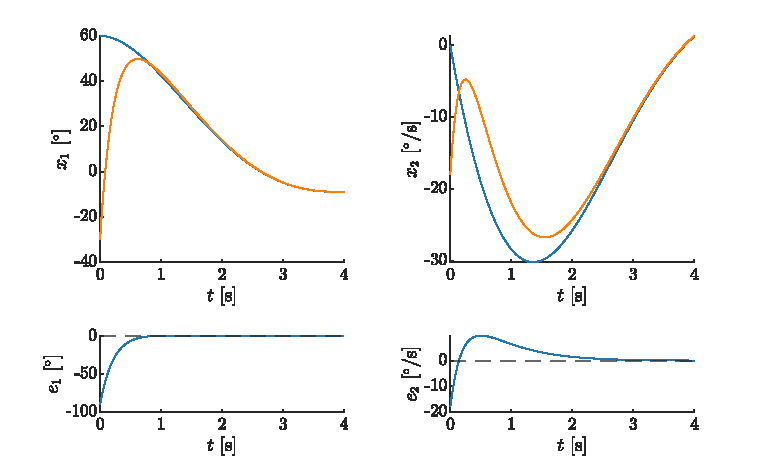
\includegraphics{figures/ex2_6.pdf}

The blue line is the true state and the orange line is estimated.

\subsection*{Code}
\subsubsection*{main system}
\begin{verbatim}
    u = @(t) 0;
    fx = @(t,x) [ x(2) ;...
                -x(2) - sin(x(1)) + u(t)];
    
    tspan = [0 4];
    y0 = [pi/3; 0];
    [t,y] = ode45(@(t,y) fx(t,y),tspan,y0);
\end{verbatim}

\subsubsection*{observer design}
\begin{verbatim}
    y_val = @(tt) interp1(t,y(:,1),tt,'spline');
    beta = 5;
    K = [beta; 1];
    fo = @(t,x) fx(t,x) + K * (y_val(t) - x(1));
    
    y0 = [-pi/6; -pi/10];
    [to,yo] = ode45(@(t,y) fo(t,y),tspan,y0);
\end{verbatim}
    
\subsubsection*{error signals}    
\begin{verbatim}
    yoo = interp1(t,y,to,'spline');
    err = (yo - yoo);
\end{verbatim}
\clearpage
\section{Le 2.8}

\subsection*{Practice}

The system:
\begin{align*}
    \dot X &= \begin{pmatrix}
        \left(\frac{x_2}{x_1}\right)^2 \\ \left(\frac{x_2}{x_1}\right)^3 - x_2
    \end{pmatrix} + \begin{pmatrix}
        x_1\\x_2
    \end{pmatrix}\,u & y = x_1\,x_2
\end{align*}
let, $z = \Phi(x) = \begin{pmatrix}
    x_1 \\ \frac{x_2}{x_1}
\end{pmatrix}$, then 
\begin{align*}
    \dot z &= \frac{\partial\Phi\left(x\right)}{\partial x}\, f\left(x,u\right)\Bigg|_{x = \Phi^{-1}(z)} = \begin{pmatrix} 1 & 0 \\ -\frac{x_2}{x_1^2} & \frac{1}{x_1}\end{pmatrix} f\left(x,u\right)\Bigg|_{x = \Phi^{-1}(z)} \\
    % &= \begin{pmatrix}
    %     \left(\frac{x_2}{x_1}\right)^2 \\ -\frac{x_2^3}{x_1^4} - \frac{x_2 - \frac{x_2^3}{x_1^3}}{x_1}
    % \end{pmatrix} + \begin{pmatrix}
    %     x_1 \\ 0
    % \end{pmatrix}\,u\Bigg|_{x = \Phi^{-1}(z)} 
    % = \begin{pmatrix}
    %     \left(\frac{x_2}{x_1}\right)^2 \\ \frac{- x_2^3 - x_1\,x_2 + \frac{x_2^3}{x_1^2}}{x_1^4}
    % \end{pmatrix} + \begin{pmatrix}
    %     x_1 \\ 0
    % \end{pmatrix}\,u\Bigg|_{x = \Phi^{-1}(z)}  \\
    &= \begin{pmatrix}
        \left(\frac{x_2}{x_1}\right)^2 \\ -\frac{x_2}{x_1}
    \end{pmatrix} + \begin{pmatrix}
        x_1 \\ 0
    \end{pmatrix}\,u\Bigg|_{x = \Phi^{-1}(z)} 
\end{align*}
it is also defined that 
\begin{align*}
    \Phi^{-1}(x) = \begin{pmatrix}
        z_1 \\ z_2\,z_1
    \end{pmatrix}
\end{align*}
Therefore, 
\begin{align*}
    \dot z &= \begin{pmatrix}
        z_2^2 \\ -z_2
    \end{pmatrix} + \begin{pmatrix}
        z_1 \\ 0
    \end{pmatrix}\,u \quad y = z_1^2\,z_2, \\
    \dot z_1 &= z_2^2 + z_1\,u \quad \dot z_2 = -z_2 \quad y = z_1^2\,z_2, \implies \dot z_1 = \frac{1}{z_1^4} z_2^2\,z_1^4 + z_1\,u \quad \dot z_2 = -z_2 \quad y = z_1^2\,z_2,
\end{align*}


\subsection*{Excercise}

The system: 
\begin{align*}
    \dot X &= \begin{pmatrix}
        x_1^2\,x_2^2 + u \\ 1 - x_1\,x_2^3 - x_2 - \frac{x_2}{x_1}\,u 
    \end{pmatrix}\quad y = x_1\,x_2 
\end{align*}
let, 
\begin{align*}
    z &= \Phi(x) = \begin{pmatrix}
        x_2x_1 \\ x_1
    \end{pmatrix}, & \implies x &= \Phi^{-1}(x) = \begin{pmatrix}
        z_2 \\ \frac{z_1}{z_2}
    \end{pmatrix}, 
\end{align*}
Then 
\begin{align*}
    \dot z &= \frac{\partial\Phi\left(x\right)}{\partial x}\, f\left(x,u\right)\Bigg|_{x = \Phi^{-1}(z)} = \begin{pmatrix} x_2 & x_1 \\ 1 & 0\end{pmatrix} \begin{pmatrix}
        x_1^2\,x_2^2 + u \\ 1 - x_1\,x_2^3 - x_2 - \frac{x_2}{x_1}\,u 
    \end{pmatrix}\Bigg|_{x = \Phi^{-1}(z)} \\
    &= \begin{pmatrix}
        x_1\,\left(1 - x_2\right) \\ x_1^2\,x_2^2 + u
    \end{pmatrix}\Bigg|_{x = \Phi^{-1}(z)} = \begin{pmatrix}
        -z_1 + z_2 \\ z_1^2 + u
    \end{pmatrix}
    % &= \begin{pmatrix}
\end{align*}   
Now, 
\begin{align*}
    y = h(x)\big|_{x = \Phi^{-1}(z)} = x_1\,x_2\big|_{x = \Phi^{-1}(z)} = z_1.
\end{align*}
Therefore, 
\begin{align*}
    \begin{pmatrix}
        \dot z_1 \\ \dot z_2
    \end{pmatrix} &= \begin{pmatrix}
        -1 & 1 \\ 0 & 0
    \end{pmatrix}\,\begin{pmatrix}
        z_1 \\ z_2
    \end{pmatrix} + \begin{pmatrix}
        0 \\ 1
    \end{pmatrix}\,u + \begin{pmatrix}
        0 \\ y^2
    \end{pmatrix} \quad y = \begin{pmatrix}
        1 & 0
    \end{pmatrix}\,\begin{pmatrix}
        z_1 \\ z_2
    \end{pmatrix}
\end{align*}
For a linear system, the observability is 
\begin{align*}
    \mathcal{O}z = \begin{pmatrix}
        C \\ C\,A
    \end{pmatrix} = \begin{pmatrix}
        1 & 0 \\ -1 & 1
    \end{pmatrix} \text{has full-column rank}
\end{align*}
If $Z$ is observable then $X$ is also observable since $X = \Phi^{-1}(Z)$, i.e., an algebraic expression.

The observer can be designed as 
\begin{align*}
\dot{\hat Z} = A\,\hat Z + f(u,y) + K\,\left(y - C\,\hat Z \right)
\end{align*}

The closed-loop observer poles 
\begin{align*}
    \alpha_\mathcal{O}(s) &= \text{det}\left(SI - A + K\,C\right) \\
    &=  \det\left(\begin{pmatrix}
        s & 0 \\ 0 & s 
        \end{pmatrix} - \begin{pmatrix}
        -1 & 1 \\ 0 & 0
    \end{pmatrix} + \begin{pmatrix}
        k_1 \\ k_2
    \end{pmatrix}\,\begin{pmatrix}
        1 & 0
    \end{pmatrix}\right)\\
    &= \det\begin{pmatrix}
        k_1 + s + 1 & -1 \\ k_2 & s
    \end{pmatrix} \\
    &= s^2 + s\,\left(k_1 + 1\right) + k_2
\end{align*}

\newpage
The width of a text is:
\printinunitsof{cm}\prntlen{\textwidth} (\printinunitsof{in}\prntlen{\textwidth}) \\
The width of a column is:
\printinunitsof{cm}\prntlen{\columnwidth} (\printinunitsof{in}\prntlen{\columnwidth}) \\
The height of a column is:
\printinunitsof{cm}\prntlen{\textheight} (\printinunitsof{in}\prntlen{\textheight}) \\ 
\end{document}
